\documentclass[oneside]{book}
\usepackage[utf8]{inputenc}
\usepackage[spanish]{babel}
\usepackage{cite,url,graphicx,epsfig,amsmath,amssymb,amsthm,appendix,authblk}
\usepackage[hidelinks,bookmarks=true]{hyperref}
\usepackage[inline]{enumitem}

\usepackage[paperwidth=17cm,paperheight=22.5cm,margin=2cm]{geometry} %dimensiones oficiales

%\setlength{\parskip}{6pt} %espacio entre párrafos
%\usepackage[letter,center,noinfo]{crop} %para revision ("frame" para cuadrito)
%\usepackage{fullpage} %otra pra revision
\newcommand{\thesisTitle}{Flujos de trabajo intensivos en datos para cómputo en la nube}

\usepackage{color} %colores para el codigo
\definecolor{mygreen}{rgb}{0,0.6,0}
\definecolor{mygray}{rgb}{0.5,0.5,0.5}
\definecolor{mymauve}{rgb}{0.58,0,0.82}

\usepackage{listings}
\usepackage{courier} %para poner codigo en monospace
%\usepackage{iconsolata}
\lstset{ %
  framextopmargin=50pt,
  backgroundcolor=\color{white},      % choose the background color
  basicstyle=\footnotesize\ttfamily,  % size of fonts used for the code
  breaklines=true,                    % automatic line breaking only at whitespace
  captionpos=b,                       % sets the caption-position to bottom
  commentstyle=\color{mygreen},       % comment style
  escapeinside={\%*}{*)},             % if you want to add LaTeX within your code
  keywordstyle=\color{blue},          % keyword style
  stringstyle=\color{mymauve},        % string literal style
  numbers=left,                       % numbering position
  escapeinside={(*@}{@*)}             % labels inside code
}
\renewcommand{\lstlistingname}{Código}
\renewcommand{\lstlistlistingname}{Lista de \lstlistingname s}


\usepackage{algorithm} % Pseudocódigo de algoritmos (Gracias Andreu)
\usepackage{algpseudocode}
\renewcommand{\algorithmicrequire}{\textbf{Entrada:}}
\renewcommand{\algorithmicensure}{\textbf{Salida:}}

%\usepackage{fixltx2e}
\MakeRobust{\Call}
%\renewcommand*\Call[2]{\textproc{#1}(#2)}

\newtheorem{defn}{Definición} %definición de definicones matemágicas

\begin{document}
%\addtocontents{toc}{Portada}
\begin{titlepage}
\begin{center}

\textsc{\underline{INSTITUTO TECNOLÓGICO AUTÓNOMO DE MÉXICO}}\\[1.5cm] % University name
%\textsc{\Large Tesis}\\[0.5cm] % Thesis type

\begin{figure}[h]
\centering
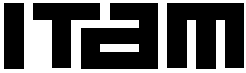
\includegraphics[scale=2]{imagenes/logoitam.png}\\[0.5cm] % Horizontal line
\end{figure} 

\huge{\thesisTitle}\\[1.5cm] % Thesis title


\large \textbf{TESIS}\\ QUE PARA OBTENER EL TÍTULO DE\\ \textbf{MAESTRO EN CIENCIAS EN COMPUTACIÓN}\\[0.8cm]
\large \textbf{P\ \  R\ \  E\ \  S\ \  E\ \  N\ \  T\ \  A}\\[0.8cm]

\textbf{FERNANDO AGUILAR REYES}\\[1.0cm]

\large ASESOR: \textbf{DR. JOSÉ OCTAVIO GUTIÉRREZ GARCÍA}\\[1.4cm]

\large \textbf{MÉXICO, D.F.} {\ \ \ \ \ \ \ \ \ \ \ \ \ \ \ \ \ \ \ \ \ \ \ \ \ \ \ \ \ \ \ \ \ \ } \textbf{2015}

\vfill
\end{center}

\end{titlepage}
 %Portada ITAM

\frontmatter
%\thispagestyle{empty}
\noindent Con fundamento en los artículos 21 y 27 de la Ley Federal del Derecho de Autor y como titular de los derechos moral y patrimonial de la obra titulada ``\thesisTitle'', otorgo de manera gratuita y permanente al Instituto Tecnológico Autónomo de México y a la Biblioteca Raúl Bailléres Jr., autorización para que fijen la obra en cualquier medio, incluido el electrónico, y la divulguen entre sus usuarios, profesores, estudiantes o terceras personas, sin que pueda percibir por tal divulgación una contraprestación.\\\\\\\\

\begin{center} 
Fernando Aguilar Reyes\\
\par\noindent\makebox[2.5in]{ }\\
\par\noindent\makebox[2.5in]{\hrulefill}\\
\par\noindent\makebox[2.5in][c]{Fecha}\\
\par\noindent\makebox[2.5in]{ }\\
\par\noindent\makebox[2.5in]{\hrulefill}\\
\par\noindent\makebox[2.5in][c]{Firma}\\
%Fecha:\\
%\rule[1em]{25em}{0.5pt} % This prints a line for the signature 
%Firma:\\
%\rule[1em]{25em}{0.5pt} % This prints a line to write the date
%}
\end{center}
\clearpage % Start a new page
 %Declaracion de derechos
%\begin{center}
Resumen
\end{center}
\noindent En este trabajo se desarroll\'o un algoritmo de planificaci\'on de flujos de trabajo con enfoque a entornos de c\'omputo en la nube, con la capacidad de calcular el número de máquinas necesarias para reducir el tiempo de espera de tareas por recursos disponibles. Tambi\'en, se implement\'o este algoritmo en un software simulador de flujos de trabajo. Los resultados experimentales muestran que el algoritmo reduce los costos de ejecuci\'on de mejor manera que los algoritmos MinMin y Miope. Por \'ultimo, se implement\'o un sistema administrador de flujos de trabajo en la nube, llamado sweeper, con el objetivo de explorar cu\'ales son los retos a los que hay que enfrentarse para llevar este tipo de algoritmos de planifcaci\'on a entornos reales.
\\\\
\noindent \emph{Palabras clave}: Planificación de flujos de trabajo, Programaci\'on din\'amica, Optimizaci\'on de costos

\begin{center}
Abstract
\end{center}
\noindent In this work we developed a workflow scheduling algorithm with a focus on cloud computing environments. This novel algorithm can compute the number of machines required to reduce task waiting time for available resources. Also, this algorithm was implemented in a workflow simulator software. The experimental results show that the algorithm reduces execution costs better than the Myopic algorithm. Finally, a prototype cloud workflow manager system, called sweeper, was developed, with the goal of exploring what are the challenges we need to face in order to use those workflow scheduling algorithms on real life scenarios.
\\\\
\noindent \emph{Keywords}: Workflow scheduling, Dynamic programming, Cost optimizacion

\clearpage
%%\addtocontents{toc}{Agradecmientos}
\begin{center}
{\huge \bfseries Agradecimientos\\}
\end{center}


A Marisela, por apoyarme en todo momento para hacer de la maestr\'ia todo un \'exito.

Al profesor Octavio Gutiérrez, por sus sabios consejos.

A Fernando Esponda y a V\'ictor Gonz\'alez, por otorgarme la opotunidad de estudiar la maestria.

A mi familia, Miguel y Florinda, Rodrigo y Mike.

A Propiedades.com, por facilitar los recursos tecnol\'ogicos para realizar este trabajo.

\tableofcontents
\listoffigures
\lstlistoflistings

\mainmatter
\chapter{Introducción}

El mundo digital dominado por datos requiere la utilización de algoritmos, tecnologías y mecanismos que permitan orquestar procesamientos de grandes volúmenes de datos, los cuales pueden tardar horas e, incluso, días en completarse. Aún así, el diseño de la aplicación junto con el flujo de trabajo que modela las tereas llevadas a cabo por la aplicación, requiere un esfuerzo considerable.

Ahora bien, sería deseable desarrollar una plataforma que permita distribuir estos flujos de trabajo computacionalmente intensivos en un sistema distribuído con el fin de disminuir el tiempo de ejecución del flujo. También, es deseable disminuir el presupuesto utilizado, ya que en la actualidad, es muy común utilizar servicios de cómputo, en el cual se paga por este servicio de acuerdo a un modelo económico en el que se paga sólo por el servicio utilizado.

En este trabajo se muestra el desarrollo de esta plataforma de ejecución de flujos de trabajo intensivo en datos con aplicación en cómputo en la nube. También se muestra el marco teórico necesario para el desarrollo de este proyecto.

Primero, empezaremos por describir el modelo de costos de cómputo en la nube, marcado por acuerdos de nivel de servicio, y se describirá un mecanismo para poder estimar el tiempo de ejecución del flujo de trabajo, necesario para poder estimar el prespuesto utilizado para ejecutar el flujo de trabajo. 

% Luego, describiremos cómo hacer benchmarking dentro de plataformas de cómputo en la nube. Se sugiere utilizar el benchmark proporcionado por LINPACK, ya que éste puede aproximar el rendimiento de un sólo núcleo y varios núcleos. En la tesis de XXX et al. se puede mostrar. Luego describiremos el algoritmo de planificación de flujos de trabajo. Luego describiremos el mecanismo para poner las tareas en de. Luego, compararemos con soluciones existentes como Aneka, HTCondor y Pegasus.


\section{Descripción del problema}

Se tiene un flujo de trabajo definido por $W = (T, D)$, donde $T$ es el conjunto de tareas del flujo de trabajo y $D$ es el conjunto de dependencias que existen entre las tareas del flujo de trabajo. Se desea planificar las tareas en un conjunto de recursos $R$ en la nube de diferente capacidad, los cuales están conectados entre sí por medio de una red privada virtual. Se tiene una función $F: W \times R \mapsto (\mathcal{R}^{+} \times {R}^{+}) $ la cual asocia un costo y un tiempo total de ejecución a una planificación de este flujo de trabajo con el conjunto de recursos dato. Se requiere minimizar la función $F$ tanto en costo como en tiempo. Cabe aclarar que, a diferencia del problema clásico de planificación de flujos de trabajo donde se tiene


\section{Lineamientos de diseño}

Desarrollar un sistema de administración de flujos de trabajo es como desarrollar una receta para hacer chocolate: hay muchas formas y modalidades de hacerlo. Sin embargo, se pueden ver algunos patrones de uso o generalidades que quisiéramos observar en el sistema administrador de flujos de trabajo. A continuación, se listarán los lineamentos de diseño deseables en el sistema administrador de flujos de trabajo.



\subsection{El flujo como centro de la aplicación}

Los sistemas de cómputo distribuido tienen inherentes una complexidad que crece más conforme mayores capacidades de agregan a éstos. Los científicos y personas especialistas de algún dominio de conocimiento cada vez tienen menos tiempo para aprender los detalles del funcionamiento de estos sistemas distribuidos. Por otro lado, dibujar diagramas que describan la secuencia de ejecución de los programas es más intuitivo. Y un flujo de trabajo bien puede expresarse a través de estos diagramas. De esta forma, especificar el flujo de trabajo es el pilar que describe los procesos a ejecutar. Por otro lado, el flujo de trabajo aporta información que ayuda a la paralelización y ejecución distribuida del mismo.



\subsection{Orientado a nubes}

Aunque se pueden ejecutar Open Grid Scheduler, HTCondor, programas MPI y aplicaciones basadas en MapReduce y cómputo distribuido en gráficas, éstos funcionan muy bien en entornos de una sola computadora con gran capacidad o en grids institucionales. Sin embargo, cuando se utilizan estos programas en enfoques como la nube, surgen algunas eventualidades, a saber: 1) es más difícil supervisar estos entornos por el hecho de la insfraestrucutra no es \emph{on-premise} o, en el caso de grids comunitarios, se conoce a ciencia cierta el funcionamiento del sistema y, 2) hay un costo monetario por utilizar estos recursos que está explícitamente establecido, el cual es deseable minimizar. Además, otra característica importante de la nube, a saber, la utilización de máquinas virutales, hace que el rendimiento del sistema distribuido en general pueda escalarse prácticamente sin límites. Por ello, es deseable ejecutar el flujo de trabajo en el menor tiempo posible, respetando un presupuesto asignado. Esta flexibilidad sólo es posible encontrarla actualmente en las infraestructuras de servicios de cómputo en la nube. Por esta razón, el sistema administrador de flujos de trabajo tiene que estar fuertemente orientado a trabajar en la nube.



\subsection{Intensivo en datos}

Como se ha dicho en la introducción, las cargas de trabajo que administran estos sistemas usualmente generan enormes cantidades de datos, que son desde logs de operación, archivos intermedios de resultados o volcados de memoria en caso de que ocurra algún error. Así, manejar datos es primordial en nuestra solucíón. Este requerimiento se puede cumplir utilizando sistemas de archivos distribuidos con énfasis en la tasa de rendimiento de datos guardados.


\subsection{Portable entre nubes}

Esto con el fin de tener la libertad de escoger la plataforma de cómputo en la nube conveniente a las necesidades del flujo.
%Aunque dudo que este requerimiento pueda cumplirse, debido a las abstracciones necesarias que deben hacerse en el software


\subsection{Simple}

Las interacciones con el usuario deben ser simples



\subsection{Basado en estándares}

\chapter{Teoría de planificación}
\label{chap:scheduling_teory}

\section{Introducción}
\label{secc:intro}

Cada día utilizamos aplicaciones de cómputo más complejas que resuelven problemas más complicados que involucran el procesamiento de grandes volúmenes de datos o contenido multimedia, demandando cada vez más poder de cómputo. Por ejemplo, hay instituciones financieras que necesitan procesar millones de transacciones diariamente; así, utilizan aplicaciones que durante el día guardan las operaciones bancarias y en la noche ejecutan estas operaciones en lotes para actualizar las cuentas bancarias. En la Bolsa Mexicana de Valores, el motor de negociación transaccional, MoNeT, puede procesar hasta 100,000 transacciones por segundo \cite{bmv2012informe}. Un último ejemplo son los proyectos de cómputo científico: éstos requieren hacer numerosos cálculos para llegar a resultados pertinentes. Tal es el caso del descubrimiento del bosón de Higgs en el Gran Colisionador de Hadrones (LHC) de la Organización Europea para la Investigación Nuclear. Se estima que cada año, el detector principal del LHC genera 15 petabytes de datos que requieren ser analizados \cite{shiers2007worldwide}. %(aproximadamente $15 \times 10^{15}$ bytes)

En cualquiera de los casos anteriores, es deseable distribuir la ejecución de estos flujos de trabajo entre varios recursos computacionales. Si bien es posible paralelizar algunos pasos de la ejecución de los flujos de trabajo, hay restricciones de orden que se deben respetar, por lo cual, es indispensable \emph{planificar} la ejecución del flujo de trabajo entre los múltiples recursos computacionales.

Definimos la \emph{planificación} como una función que asigna a cada tarea del flujo de trabajo un servicio que contiene los recursos para ejecutar dicha tarea, con el fin de completar la ejecución de todas las tareas de manera satisfactoria, cumpliendo ciertas restricciones \cite{wieczorek2009towards}, por ejemplo, restricciones de orden de ejecución. Con ello, se desea encontrar una forma óptima de hacer esta planificación para reducir el tiempo de ejecución total del flujo de trabajo. Sin embargo, con la aparición del cómputo en la nube, es posible ejecutar nuestro flujo de trabajo con otras restricciones, como minimizar el presupuesto necesario para la ejecución del flujo afectando el tiempo de ejecución.

Sin embargo, aún no existe un consenso general sobre cuál es una definición completa de un flujo de trabajo \cite{van2003workflow}, debido a que los sistemas que administran y ejecutan las tareas de un flujo de trabajo utilizan especificaciones diferentes para expresar el flujo de trabajo. También, esta falta de consenso da lugar a que un flujo de trabajo pueda ser interpretado desde varias perspectivas, es decir, un flujo de trabajo puede representar dependencias de datos o dependencias de orden entre las tareas. Así, es necesario establecer una base para representar los flujos de trabajo, y con ello, diseñar algoritmos de planificación de flujos de trabajo que puedan ser utilizados en ambientes de cómputo distribuidos. Finalmente, es deseable que estos algoritmos de planificación optimicen el tiempo de ejecución total del flujo de trabajo o que ajusten la ejecución del flujo a un limitado presupuesto de recursos.

% La organización del documento es la siguiente: en la sección \ref{secc:definitions} se define formalmente el problema de planificación de flujos de trabajo. En la sección \ref{secc:taxonomy} se presenta una taxonomía de los algoritmos de planificación de flujos de trabajo. En la sección \ref{secc:simulation} se proporcionan detalles de un simulador de ejecución de flujos de trabajo propuesto en este artículo. En la sección \ref{secc:related} se describen taxonomías similares y plataformas para ejecutar flujos de trabajo. Finalmente, en la sección \ref{secc:conclusions} se presentan algunas conclusiones.



\section{Flujos de trabajo y el problema de planificación} 
\label{secc:definitions}

La \emph{planificación} es el proceso de asignación de recursos a tareas, de tal modo que se define un orden de ejecución de las tareas, teniendo lugar diferentes combinaciones de recursos y tareas. Primero se definirá de la forma más elemental el problema de la planificación para estudiar sus propiedades y con ello, explicar la relación de este problema fundamental con el problema de planificación de flujos de trabajo. Esto nos permitirá enunciar una propiedad importante del problema de planificación de flujos de trabajo, a saber: este problema pertenece a la clase de complejidad NP-completo.


\subsection{El problema fundamental de la planificación}
De acuerdo a  Ullman et al. \cite{ullman1975np}, el \emph{problema fundamental de la planificación} está compuesto por:
 
\begin{enumerate}
\item Un conjunto de tareas $\mathcal{J} = \{ J_1, J_2, \dots, J_n \}$
\item Un ordenamiento parcial $\prec$ sobre $\mathcal{J}$
\item Una función de costo $U: \mathcal{J} \mapsto \mathbb{Z}^{+}$, la cual indica el tiempo que tarda en completarse cada una de las tareas de $\mathcal{J}$
\item Un número de computadoras (procesadores) $k$
\end{enumerate}

En el trabajo de Ullman et al. \cite{ullman1975np}, el objetivo del problema fundamental de la planificación es \emph{minimizar} el tiempo total de ejecución, denotado por $t_{max}$, respetando el orden parcial definido por $\prec$, asignando tareas de $\mathcal{J}$ a los $k$ procesadores. También, es importante notar que se asume que cuando una computadora ejecuta una tarea, ésta es ejecutada completamente, sin errores o interrupciones.

Como puede notarse, hay varias maneras de acomodar las $k$ computadoras para que se ejecuten todas las tareas de $\mathcal{J}$. De hecho, Ullman et al. han demostrado que este problema pertenece a la clase de complejidad NP-completo \cite{ullman1975np}. Esto significa que no se ha encontrado un algoritmo que pueda resolver el problema en tiempo polinomial. Entonces, la solución ingenua de probar ordenadamente todas las posibles asignaciones de tareas a computadoras resulta computacionalmente muy costosa.


\subsection{Planificación de flujos de trabajo}

Para plantear el problema de la planificación de flujos de trabajo, primero se mostrará que, bajo ciertas condiciones, un flujo de trabajo puede ser reducido a un grafo dirigido acíclico haciendo las transformaciones adecuadas. Luego, se utilizará la definición del problema básico de planificación con restricciones y su semejanza para flujos de trabajo. Finalmente, se hará una descripción de la complejidad de planificar flujos de trabajo.


\subsubsection{Reducción de flujos de trabajo a grafos dirigidos acíclicos.}

En el trabajo de Mair et al. \cite{mair2007workflow} se propone un formato para una representación intermedia de flujos de trabajo basada en grafos dirigidos acíclicos, con el fin de transformar una especificación detallada de un flujo de trabajo, escrita en un lenguaje basado en XML llamado AGWL, a esta representación intermedia. De acuerdo a lo discutido anteriormente en la sección \ref{secc:intro} de este documento, un flujo de trabajo puede ser interpretado desde varias perspectivas. Sin embargo, un grafo dirigido acíclico resume en pocos elementos (nodos y aristas) las tareas y las dependencias que deben ser cumplidas durante la planificación. Es por esta razón que es deseable reducir un flujo de trabajo, interpretado desde cualquier perspectiva, a un grafo dirigido acíclico.

Además, aún no existe un consenso sobre qué representa un flujo de trabajo \cite{van2003workflow}, debido a las diferentes perspectivas de su interpretación. En el caso del lenguaje AGWL, éste cuenta con facilidades para poder expresar flujos de trabajo condicionales, a saber: construcciones \texttt{if}, \texttt{while}, \texttt{for} y \texttt{parallel}. Estas facilidades permiten expresar una gran variedad de flujos de trabajo. Sin embargo, para poder estudiar los flujos de trabajo con estas construcciones, se requieren de mecanismos de predicción o estimación de posibles rutas de ejecución del flujo de trabajo. Por esta razón, el estudio de estos mecanismos está fuera del alcance de este trabajo, restringiendo el estudio a flujos de trabajo con ejecución atómica (sin fallos) y sin estructuras condicionales.

\subsubsection{Definición del problema de planificación de flujos de trabajo.}
Una vez que se ha establecido a los grafos dirigidos acíclicos como nuestra representación básica de flujos de trabajo, se definirá el problema que conlleva asignar recursos a las tareas del flujo. Con el fin de no perder generalidad, tomaremos las definiciones de Wieczorek-Prodan \cite{wieczorek2008taxonomies} para definir el problema de la planificación de flujos de trabajo:

\begin{defn}
Un \textbf{flujo de trabajo} es un grafo dirigido acíclico $w \in \mathcal{W}, w = (\mathcal{V},\mathcal{E})$, compuesto de un conjunto de nodos $\mathcal{V}$ que representan tareas $ \tau \in \mathcal{T}$ y un conjunto de aristas $\mathcal{E}$ que representan transferencias de datos $ \rho \in \mathcal{D}$.
\end{defn}

\noindent Hay que notar en la definición anterior que la forma en que se relacionan las tareas y las transferencias de datos con los nodos y aristas del grafo está determinada por la representación del flujo de trabajo, es decir, las aristas representan tanto dependencias de datos como restricciones de orden de las tareas. Ahora se definirán los recursos de cómputo en donde se ejecuta el flujo.
%\emph{concreta}
%creo que esto requiere más trabajo.
%La definición de Wieczorek-Prodan habla de grids, pero es fácilmente aplicable a otros enfoques de cómputo.

\begin{defn}
Un \textbf{servicio} es una entidad de cómputo que puede ejecutar una tarea $\tau \in \mathcal{T}$. El conjunto de todos los servicios disponibles para ejecutar el flujo de trabajo está denotado por $\mathcal{S}$.
\end{defn}

\noindent De este modo, se puede definir la planificación como una regla de asociación entre servicios y tareas del flujo de trabajo:

\begin{defn}
La \textbf{planificación de un flujo de trabajo} $w$ es una función $ f: \mathcal{T} \mapsto \mathcal{S}$ que asigna servicios a las tareas del flujo. El conjunto que contiene todas las posibles planificaciones de $w$ es denotado por $\mathcal{F}$.
\end{defn}

\noindent Cada posible planificación determina un costo de ejecución. A continuación, definiremos el modelo de costos determinado por la utilización de los servicios.

\begin{defn}
Un \textbf{modelo de costos} $C = \{c_1, \dots, c_n\}$ es un conjunto de criterios que determinan las restricciones en las que se debe ejecutar una planificación, por ejemplo, un límite en el tiempo de ejecución, en el costo monetario o la tolerancia a fallos, entre otros.
\end{defn}

\begin{defn}
Para cada criterio $c_i \in C$, existe una \textbf{función de costo parcial} $\Theta_i : \mathcal{S} \mapsto \mathbb{R}$, en la que a cada servicio disponible para ejecutar el flujo de trabajo se le asocia un costo por ejecutar dicho servicio con las restricciones dictadas con el criterio $c_i$.
\end{defn}

\noindent Las funciones de costo parcial son útiles para determinar costos a nivel de tareas; es decir, con una función de costo parcial podemos definir el tiempo que tomará ejecutar una tarea en un recurso determinado o el costo monetario de ejecutar la tarea en dicho recurso.

\begin{defn}
Para cada criterio $c_i \in C$, existe una \textbf{función de costo total} $\Delta_i : \mathcal{W} \times \mathcal{F} \mapsto \mathbb{R}$, que asigna un flujo de trabajo $w$ planificado por $f$ un costo basado en los costos parciales determinados por los servicios utlizados para ejecutar las tareas del flujo.
\end{defn}

\noindent Por lo tanto, el objetivo del problema de la planificación de flujos de trabajo es encontrar la planificación $f$ que minimice las funciones de costo total $\Delta_i$, $1 \le i \le n$.

\subsubsection{Complejidad computacional de la planificación de flujos de trabajo.}
%Después de haber enunciado varias definiciones para definir el problema de la planificación de flujos de trabajo
Ahora, se hará una equivalencia con el problema fundamental de planificación visto anteriormente para estudiar su complejidad computacional. La equivalencia es la siguiente:

\begin{enumerate}
\item El conjunto de tareas $\mathcal{J}$ equivale a las tareas $\mathcal{T}$ descritas por el flujo de trabajo.

\item El ordenamiento parcial $\prec$ está representado tanto por las dependencias de datos $\mathcal{D}$ y las aristas $\mathcal{E}$ que representan el control de flujo que deben respetarse para ejecutar el flujo.

\item Las $k$ computadoras equivalen al conjunto de servicios $\mathcal{S}$ disponibles para ejecutar el flujo.

\item La función de costo $U$ tiene una equivalencia implícita. El problema fundamental asume que conocemos apriori el tiempo de ejecución de una tarea. Sin embargo, es muy frecuente que sólo tengamos una estimación del tiempo de ejecución. Por otro lado, podemos establecer una función auxiliar que relacione las tareas con los servicios. Dicha relación es la función de planificación $f$. En efecto, ejecutar una tarea en un servicio genera un costo, determinado por las funciones parciales y totales. Así, estableceremos una relación proporcional entre costo y tiempo, con el fin de mostrar que existe una equivalencia entre la función de costo $W$ del problema fundamental y el modelo de costo de un flujo de trabajo.
\end{enumerate}

Con lo anterior, se ha mostrado que el problema de la planificación de flujos de trabajo es equivalente al problema fundamental de planificación. Entonces, se puede inferir que el problema de la planificación de flujos de trabajo pertenece a la clase de complejidad NP-completo.



\section{Taxonomía de los algoritmos de planificación de flujos de trabajo}
\label{secc:taxonomy}

Como han aparecido numerosos algoritmos para planificar flujos de trabajo, es natural que surjan clasificaciones \cite{topcuoglu2002performance} \cite{yu2008workflow} para tener una mejor idea de los avances logrados en este tema y los puntos clave con los que trabajan los algoritmos.

De acuerdo a Yu et al. \cite{yu2008workflow}, se pueden clasificar los algoritmos de planificación de flujos de trabajo ejecutados en grids en dos grandes niveles: 1) los algoritmos de mejor esfuerzo y 2) los algoritmos de calidad en el servicio. Al primer grupo pertenecen aquellos algoritmos que tratan de minimizar el tiempo total de ejecución\footnote{También conocido como \emph{makespan}}, haciendo uso de todos los recursos disponibles. En el segundo grupo, los algoritmos tratan de obtener una planificación que cumpla las restricciones especificadas como una medida de calidad, con la posibilidad de elegir soluciones que tomen un tiempo de ejecución subóptimo. A su vez, cada grupo tiene ramas de clasificación. En la figura \ref{fig:taxonomy} se puede visualizar la taxonomía.

\begin{figure}
\begin{center}
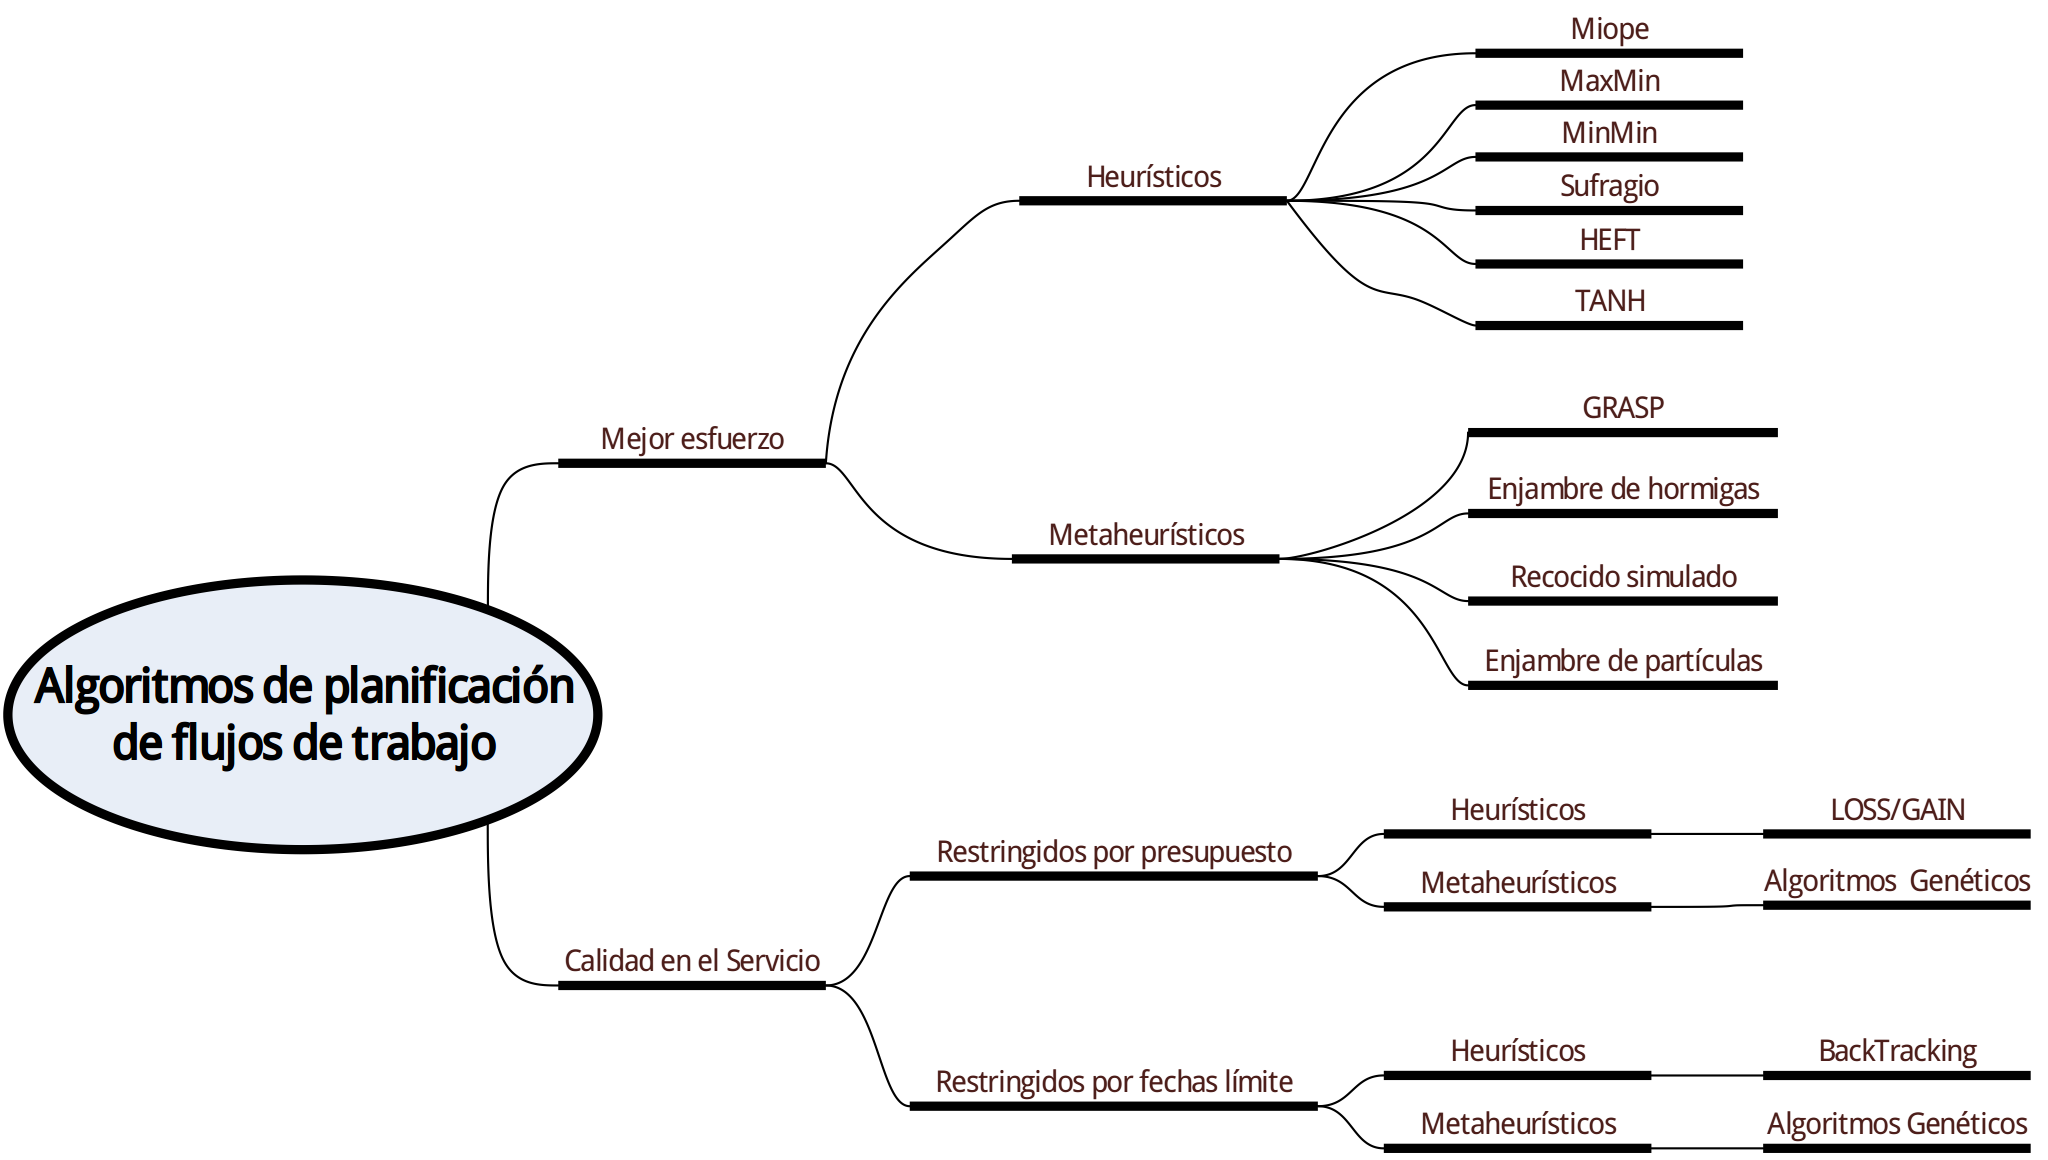
\includegraphics[width=1.0\textwidth]{imagenes/taxonomy}
\end{center}
\caption{Diagrama de la taxonomía de los algoritmos de planificación de flujos de trabajo.}
\label{fig:taxonomy}
\end{figure}

%A continuación, mostraremos los algoritmos descritos en la clasificación de Yu et al.: %con los ajustes en notación necesarios para que coincidan con las definiciones de flujo de trabajo establecidas en el capítulo anterior.


\subsection{Algoritmos de mejor esfuerzo}
%o \emph{makespan}
Estos algoritmos tratan de minimizar algún criterio, que en muchos casos es el tiempo total de ejecución. Cabe aclarar que para los siguientes algoritmos, se asumirá que el grafo del flujo de trabajo tiene una correspondencia biyectiva entre los nodos $\mathcal{V}$ y las tareas $\mathcal{T}$, es decir, cada nodo del grafo representa una tarea del flujo de trabajo. Las aristas del grafo representan \emph{dependencias entre tareas}.

También, los algoritmos de mejor esfuerzo se pueden dividir en algoritmos guiados por heurísticas y en algoritmos guiados por metaheurísticas. El primer subgrupo debe su nombre a que las soluciones están basadas en ideas que resuelven de manera aproximada el problema de la planificación bajo ciertas condiciones \cite{yu2008workflow}. El segundo subgrupo contiene a los algoritmos que utilizan algún método para elegir o generar planificaciones que se acerquen al óptimo.

\subsubsection{Algoritmos heurísticos de mejor esfuerzo.}

Los algoritmos heurísticos se pueden dividir en cuatro grandes tipos: 
\begin{enumerate*}[label=\alph*)]
\item{algoritmo inmediato,}
\item{algoritmos basados en lista,}
\item{agrupamiento de tareas y}
\item{duplicación de tareas.}
\end{enumerate*}

En el primer grupo se encuentra el algoritmo Miope \cite{ramamritham1990efficient}, que sólo asigna tareas a recursos conforme se va necesitando. Los algoritmos basados en lista, como MaxMin, MinMin y Sufragio \cite{maheswaran1999dynamic}, ordenan las tareas de acuerdo a algún criterio (fase de priorización) y seleccionan las tareas de acuerdo a cierto criterio (fase de selección). En el caso de los algoritmos de agrupamiento de tareas, tales como TANH \cite{bajaj2004improving}, al inicio, crean un conjunto para cada tarea. Después, con un paso de mezcla se van uniendo conjuntos hasta que quede un número de conjuntos igual al número de recursos disponibles. Finalmente se ordenan las tareas de cada conjunto para ejecutarse en cada recurso. Por último, los algoritmos de duplicación de tareas (Híbrido \cite{sakellariou2004hybrid}, TANH \cite{bajaj2004improving}) planifican una tarea en varios recursos con el fin de reducir el costo por comunicación entre recursos; cada uno de estos algoritmos se caracteriza por la manera en que eligen las tareas a planificar.


\subsubsection{Algoritmos metaheurísticos de mejor esfuerzo.}

Estos algoritmos son clasificados de acuerdo a la metaheurística que utilizan. Para esta clasificación, vamos a describir cuatro tipos de metaheurísticas: 
\begin{enumerate*}[label=\alph*)]
\item{algoritmos genéticos,}
\item{búsqueda aleatoria adaptativa dirigida --GRASP--,}
\item{recocido simulado y}
\item{optimización por enjambre de partículas}
\end{enumerate*}

Los algoritmos genéticos simulan el proceso de selección natural con posibles planificaciones e introducen mutaciones para evitar enfocarse en una solución local. Con la ayuda de una función de evaluación (\emph{fitness}), se mide la calidad de la planificación y se eligen aquellas soluciones que resulten mejor evaluadas \cite{yu2006scheduling}. El algoritmo GRASP \cite{blythe2005task} genera aleatoriamente soluciones y con un procedimiento voraz\footnote{Greedy} elige las soluciones óptimas locales \cite{blythe2005task}. El recocido simulado, como su nombre lo indica, emula el proceso de formación de cristales donde en cada iteración se va creando una mejor solución \cite{young2003scheduling}. Finalmente, la optimización por enjambre de partículas representa una posible planificación como un punto en el espacio y el algoritmo hace que las mejores soluciones cambien su posición de acuerdo a una velocidad que es proporcional a la calidad de la solución \cite{wu2010revised}.


\subsection{Algoritmos de calidad en el servicio}

En estos algoritmos, se definen un conjunto de restricciones que debe respetar la planificación. Principalmente, estas restricciones tienen que ver con un presupuesto global limitado y un límite en los tiempos de ejecución total del flujo de trabajo. También es posible definir límites de tiempo de ejecución o límites de presupuesto para cada tarea particular del flujo.

De acuerdo a la forma que trabajan estos algoritmos, pueden dividirse en: restringidos por presupuesto o restringidos por fecha límite. Los primeros son algoritmos que utilizan el presupuesto para cumplir con restricciones de calidad del servicio. Los algoritmos restringidos por fecha límite buscan planificaciones que cumplan con fechas proporcionadas. Ambos grupos se subdividen en heurísticos y metaheurísticos. A continuación, describiremos estas subdivisiones.


\subsubsection{Algoritmos restringidos por presupuesto.}

Los algoritmos restringidos por presupuesto se dividen en: 
\begin{enumerate*}[label=\alph*)]
\item{heurísticos y}
\item{metaheurísticos.}
\end{enumerate*}

En la primera división se encuentran los algoritmos que trabajan con una idea base que genera soluciones que no están garantizadas que sean óptimas. En este grupo de algoritmos se encuentra el algoritmo LOSS/GAIN, propuesto por Tsiakkouri et al. \cite{sakellariou2007scheduling}. Los algoritmos metaheurísticos generan soluciones aleatoriamente y utilizan la información de iteraciones pasadas para refinar las soluciones. En el trabajo de Yu et al. \cite{yu2006scheduling} se propone un algoritmo genético cuya función de evaluación valora mejor a las planificaciones que cumplan con el presupuesto con un tiempo de ejecución mínimo.


\subsubsection{Algoritmos restringidos por fechas límites.}

Los algoritmos restringidos por fechas límites también se dividen en:
\begin{enumerate*}[label=\alph*)]
\item{heurísticos y}
\item{metaheurísticos.}
\end{enumerate*}

En el primer grupo se encuentran el algoritmo BackTracking, propuesto por Menascé et al. \cite{menasce2004framework}, y el algoritmo de distribución de fechas límite, propuesto por Yu et al. \cite{yu2005cost}. En el segundo grupo se encuentra un algoritmo genético presentado en \cite{yu2006scheduling}, cuya función \emph{fitness} valora mejor a aquellas soluciones que cumplan con la fecha límite, con un presupuesto mínimo.

	
\subsubsection{Estimación del tiempo.}

En estos algoritmos se asume que se conoce el tiempo de ejecución de las tareas del flujo de trabajo. Sin embargo, en la etapa de diseño de un flujo de trabajo, es complicado conocer la duración de las tareas, debido a que son muchos los factores que influyen el tiempo total de ejecución del flujo, como el rendimiento de la plataforma de cómputo, la cantidad de datos a procesar, el tiempo de comunicación entre nodos de cómputo, entre otros factores. Para mitigar este problema, se han hecho algoritmos basados en series de tiempo que estiman el tiempo de ejecución de cada una de las tareas de un flujo de trabajo. Estos algoritmos utilizan información histórica de ejecuciones de flujos de trabajo para realizar las predicciones  \cite{liu2011novel}.

\chapter[Algoritmos]{Flujos de trabajo sobre cómputo en la nube}
\label{chap:algorithm}

En este capítulo, describiremos el algoritmo que es la pieza clave del sistema para agendar tareas de un flujo de trabajo en infraestructura de cómputo en la nube, tomando en cuenta los lineamientos de diseño propuestos anteriormente.



\section{Antecedentes}

Un área de investigación activa es la planificación de tareas a nivel de procesador (CPU's), en donde se asume que se tiene un procesador cuyos núcleos son idénticos e intercambiables. En los trabajos de investigación referentes a esta área se consideran a los grafos dirigidos acíclicos como los modelos de tareas más generales. Así, en el trabajo de Saifullah et al. \cite{saifullah2013multi}, se transforma un grafo dirigido acíclico en un conjunto de tareas secuenciales con secciones que se ejecutan en paralelo.


% Podemos hacer esto aún más abstracto y combinarlo con la teoría de Pinedo

% EFT: Earliest-Finish Time
% DM: Deadline Monotonic
% EDF: Earliest-Deadline First
% Global EDF
% Partitioned EDF

% how to enable theory with processor teory
% I think my thesis is that weird link, with the basic paper
% no hay que olvidar que hay que optimizar tiempo, dinero

% ya sabemos que es NP-hard, asi que nos enfocaremos en el problema

% Primero, tienes recursos 'infinitos', solo sujetos a presupuesto
% puedes averiguar el numero maximo de maquinas a levantar con el modelo de tareas paralelar
% simplemente cuentas el segmento con el mayor numero de paralelizaciones

Es muy común que los servicios de cómputo en la nube se pague la utilización de las máquinas virtuales por hora, dejando sin cobrar porciones de hora no utlizadas. Además, se pueden solicitar tantos recursos como se requieran, limitándose solamente al presupuesto disponible. Tambi\'en, estas máquinas virtuales son recursos variados; pueden ser desde máquinas con un solo procesador, hasta m\'aquinas virtuales con grandes cantidades de memoria y m\'ultiples procesadores.

De acuerdo al primer cap\'itulo del libro de Pinedo \cite{pinedo2012scheduling} hay esfuerzos para clasificar los problemas de planificación en general. Sin embargo, la clasificación presentada en este trabajo sólo contempla los problemas que optimizan una sola métrica, aunque, se puede utilizar una combinación de funciones objetivo a optimizar. Sin embargo, esta forma de atacar el problema de planificación multiobjetivo no garantiza evaluar todas las posibles opciones. 

% Hacer puente entre las teorías de Buyya y Jia Yu y las teorías de Pinedo

% Hay que leer los papers de arquitectura

\section{Los cuatro algoritmos}

Si bien en la literatura hay múltiples algoritmos de planificación publicados por la comunidad científica, éste es sólo una parte (muy importante) de un sistema administrador de flujos de trabajo. En el caso de este trabajo, dividimos todo el proceso en cuatro fases:

\begin{enumerate}
\item{Planificación}
\item{Asignación de recursos}
\item{Ejecución}
\item{Descarga de resultados}
\end{enumerate}



\subsection{Planificación}

La idea base del algoritmo es lidiar con las dependencias, ya que éstas generan restricciones sobre el problema. Otra característica a aprovechar es el hecho de que los recursos de cómputo en la nube pueden ser tratados como \emph{efímeros}, es decir, pueden ser creados y destruidos conforme se requiera.

De esta forma, el primer paso del algoritmo de planificación es dividir el flujo de trabajo en segmentos consecutivos, con la propiedad de que un segmento sólo dependa de la ejecución completa del segmento anterior.

Para generar los segmentos, se utiliza la definición de Saifullah et. al \cite{saifullah2013multi} basada en la profundidad de cada nodo del grafo dirigido ac\'iclico que representa el flujo de trabajo.

\begin{defn}

La \textbf{profundidad} $h$ de una tarea $t$ de un flujo de trabajo está definida como:

\begin{displaymath}
h(x) = \left\{
     \begin{array}{lr}
       \max_{u \in \text{Padres}(t) } h(u) + 1 & : | \text{Padres}(t) | \neq 0 \\
       1                                       & : | \text{Padres}(t) | = 0
     \end{array}
   \right.
\end{displaymath}

\noindent Donde $\text{Padres}(t)$ es el conjunto de tareas que inmediatamente preceden a la tarea $t$, es decir, aquellas tareas $u$ que tienen una dependencia de orden que va a la tarea $t$.
\end{defn}

En la figura \ref{fig:DAG_to_segment} se puede apreciar un ejemplo de este algoritmo, en donde se puede ver que a cada tarea del flujo de trabajo se le asigna un segmento, en cual se está garantizando que cada segmento sólo dependa del segmento anterior.

\begin{figure}
\begin{center}
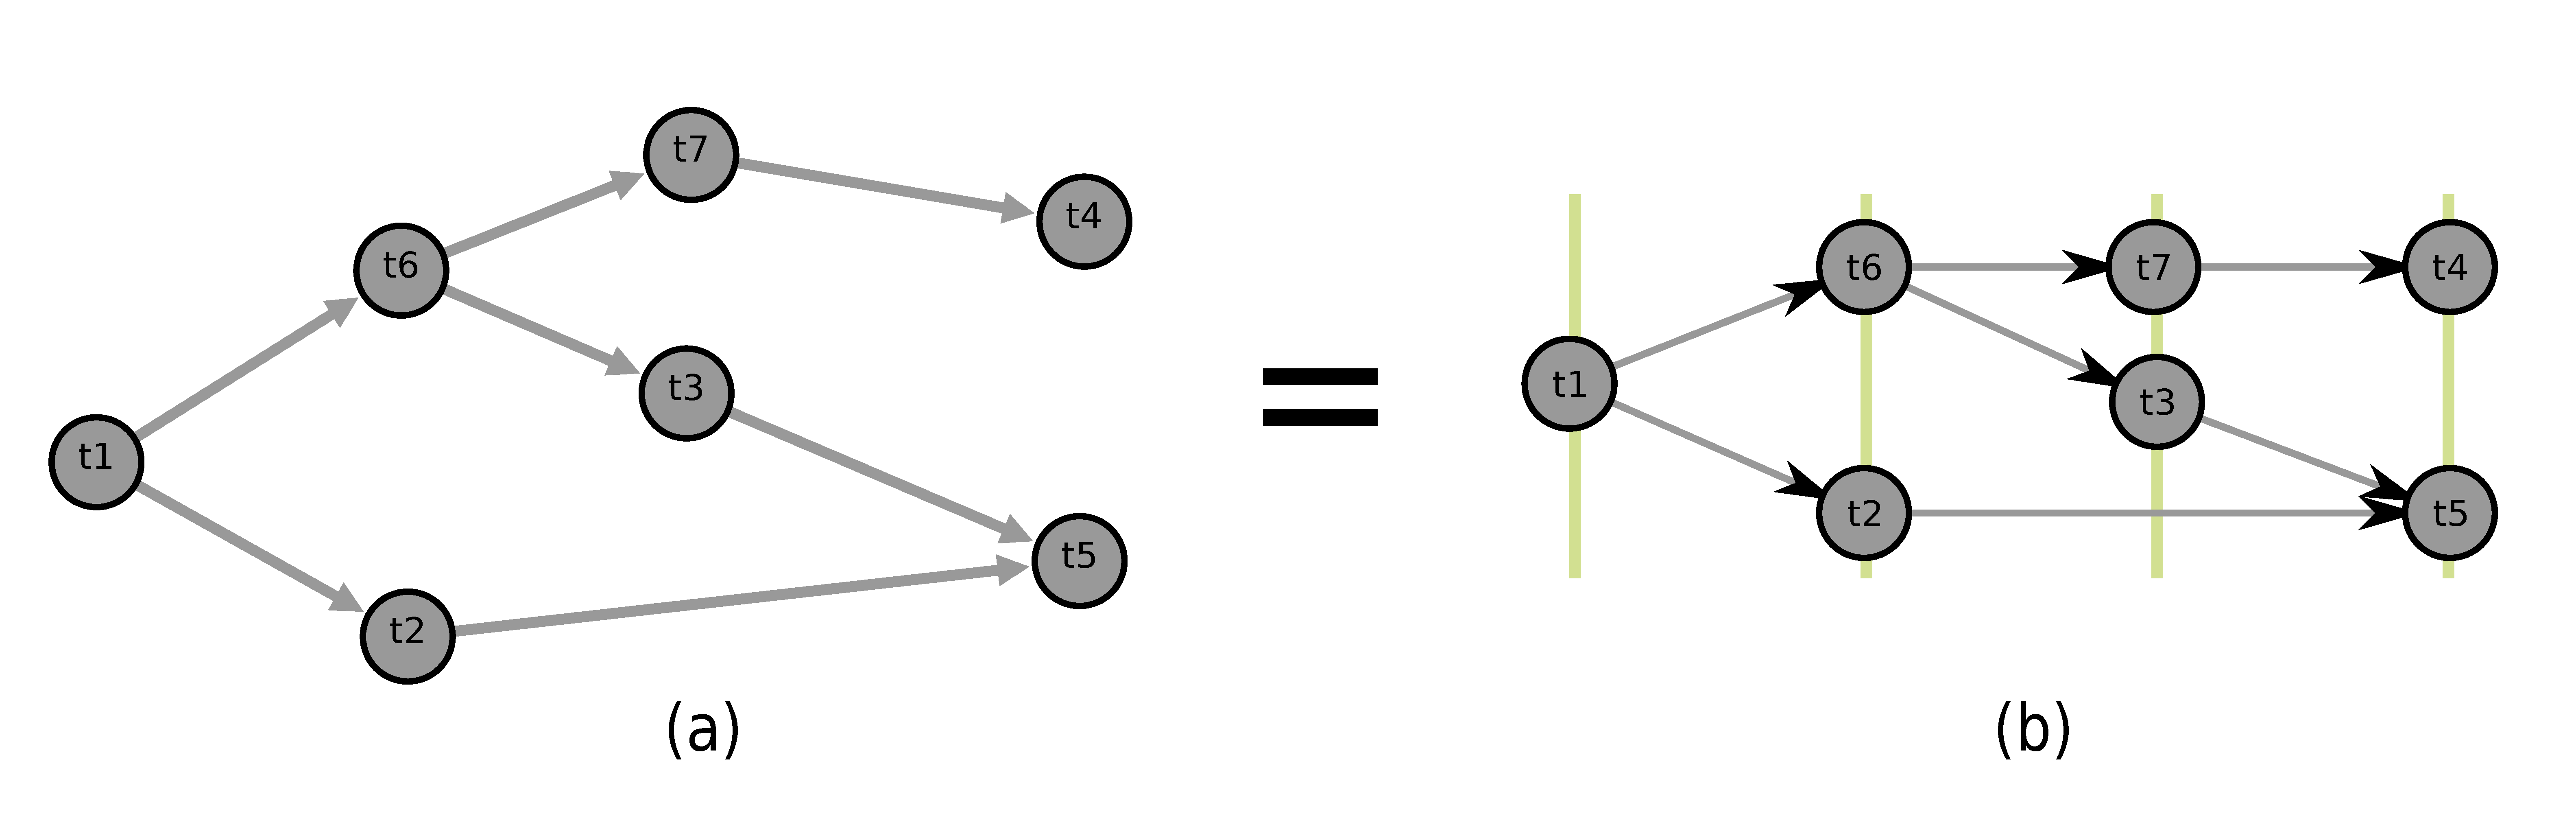
\includegraphics[width=1.0\textwidth]{imagenes/DAG_to_segment.pdf}
\end{center}
\caption{Transformación de un flujo de trabajo (a) a segmentos (b)}
\label{fig:DAG_to_segment}
\end{figure}

Otro punto a notar es que hay un límite en el número de tareas concurrentes que es posible ejecutar debido a las restricciones. Esto implica que a lo sumo hay un número finito de recursos concurrentes que se necesitan para correr el flujo de trabajo. Este límite equivale al máximo de tareas de los segmentos que conforman el flujo de trabajo.

En el pseudocódigo \ref{alg_blind_segments}, se calculan los segmentos de un flujo de trabajo.

\begin{algorithm}
\caption{Segmentación de un flujo de trabajo}
\label{alg_blind_segments}
\begin{algorithmic}[1]
\Require{Un flujo de trabajo $workflow$}
\Ensure{Un mapa con los segmentos de cada tarea del flujo de trabajo}
\Procedure{get\_task\_segments}{$workflow$}
	\State $visited \gets$ Diccionario
	\State $segment \gets$ Diccionario
	\For{$t \in workflow.tasks$}
		\State \Call{get\_segment}{$t$}
	\EndFor
	\State \Return $segment$
\EndProcedure

\Procedure{get\_segment}{$task$}
	\State $visited[task] \gets True$
	\State $max\_seg \gets 0$
	\If{$ \lnot (task \in segment)$}
		\State $segment[task] \gets 0$
		\For{$p \in task.parents$}
			\State $v \gets \Call{get\_segment}{p}$
			\If{$v > max\_seg$}
				\State $max\_seg = v$
			\EndIf
		\EndFor
		\State $segment[task] \gets max\_seg + 1$
	\EndIf
	\State \Return $segment[task]$
\EndProcedure


\Procedure{estimate\_resources}{$workflow$}
	\State $segments \gets \Call{$get\_task\_segments$}$
	\State $segmentsHeight \gets $ Diccionario
	\State $max\_segment \gets 0$
	\For{$k$, $v$ in $segments$}
		\State $segment \gets v$
		\If{$segment \in segmentsHeight$}
			\State $val \gets segmentsHeight[ segment ]$
		\Else
			\State $val \gets 0$
		\EndIf
		\State $val \gets val + 1$
		\State $max\_segment \gets \max(val, max\_segment)$
	\EndFor
\EndProcedure
	
\end{algorithmic}
\end{algorithm}

\subsection{Asignación de recursos}

Ahora, el cómputo en la nube abre otras posibilidades que no se pueden realizar en los entornos de cómputo distribuido tradicionales, como el hecho de poder solicitar máquinas virtuales de acuerdo a la demanda. De esta forma, con las tareas del flujo de trabajo segmentadas, se puede ver a cada segmento como un conjunto de tareas independientes. Así, se puede usar un algoritmo de programación dinámica que pueda encontrar la asignación óptima de máquinas virtuales y tareas entre cada segmento.

Así, este algoritmo se puede ver como el algoritmo de la mochila \emph{inverso} con múltiples mochilas, en donde las mochilas son las posibles configuraciones y las tareas son objetos que deben ser \emph{embolsados}. El objetivo de este algoritmo es encontrar aquella asignación que pueda embolsar todas las tareas maximizando el uso del espacio de las mochilas, sujeto a una condición de optimalidad. Para este caso, la condición de optimalidad es definida a trav\'es de una funci\'on de costo parcial, especificada por el usuario. 

Por el momento, para hacer la relaci\'on entre configuraciones y tareas, se asume que cada tarea ocupa un núcleo de una máquina virtual y que todas las posibles configuraciones de máquinas virtuales del proveedor tienen memoria primaria suficiente para ejecutar las tareas.

El algoritmo de asignación de recursos a tareas de un segmento está descrito en el pseudocódigo \ref{alg_blind_main}. Como se puede notar en este pseudocódigo, hay dos funciones que son invocadas. La primera, llamada $\Call{take}{}$, calcula los costos óptimos de generar una asignación que utilice todos los n\'ucleos de las configuraciones de las máquinas virtuales. La segunda funci\'on, llamada $\Call{check\_take}{}$, reconstruye la soluci\'on \'optima que fue encontrada por la primera funci\'on'

\begin{algorithm}
\caption{Asignación de configuraciones de recursos tareas de un segmento}
\label{alg_blind_main}
\begin{algorithmic}[1]
\Require{ 
Los siguientes parámetros:
\begin{itemize}
	\item Una lista de tareas de un segmento $tasks$
	\item Una lista de configuraciones de recursos $resource\_configs$ 
\end{itemize}
}
\Ensure{Una lista de asignaciones de tarea -- recurso $resource\_mappings$}

\Procedure{bin\_packing}{$tasks$, $resource\_configs$}
	\State $mem\_costs \gets$ Matriz de $|tasks| \times |resource\_configs|$, inicializado con 0 
	\State $visited \gets$ Matriz de $|tasks| \times |resource\_configs|$, inicializado con 0
	\State $used \gets$ Arreglo de tamaño $|resource\_configs|$, incializado con $\texttt{MAX\_INT}$
	\State $resource\_mappings \gets$ Lista vacía
	\State \Call{take}{0, 0}
	\State \Call{check\_take}{0, 0}
	\State \Return $resource\_mappings$
\EndProcedure
\end{algorithmic}
\end{algorithm}


Ahora, en los pseudocódigos \ref{alg_blind_take} y \ref{alg_blind_check_take}, se muestran los procedimentos principales para generar la asignación de recursos de un segmento de tareas un flujo de trabajo. El procedimiento del pseudocódigo \ref{alg_blind_take} calcula el costo de la asignación óptima, de acuerdo a la funci\'on de costo definida por el usuario. El procedimiento del pseudoc\'odigo \ref{alg_blind_check_take} construye a partir de la tabla de costos generada por el pseudoc\'odigo anterior la asignaci\'on de recursos y tareas cuyo costo es m\'inimo.


\begin{algorithm}
\caption{Asignación óptima por búsqueda exhaustiva}
\label{alg_blind_take_exhaustive}
\begin{algorithmic}[1]
\Require{Lista de tareas y configuraciones a asignar}
\Ensure{Una asignación óptima para el segmento}
\Procedure{take\_exhaustive}{$t_i$, $rc_i$}
	\If{$rc_i = |resource\_configs|$}
		\State{\Return{$\infty$}}
	\EndIf

	\If{$t_i = |tasks|$}
		\State{\Return{\Call{checkMapping}{}}}
	\EndIf

	\State{\Call{pushEntry}{$t_i$, $rc_i$}}
	\State{$coresUsed[rc_i] \gets coresUsed[rc_i] + 1$}
	\State{$takedYes \gets \Call{take}{t_i + 1, 0}$}

	\State{$coresUsed[rc_i] \gets coresUsed[rc_i] - 1$}
	\State{\Call{popEntry}{$t_i$, $rc_i$}}
	\State{$takedNot \gets \Call{take}{t_i, rc_i + 1}$}

	\If{$takedYes = \infty \land takenNot = \infty$}
		\State{\Return{$\infty$}}
	\EndIf

	\State{\Return{$\min(takedYes, takenNot)$}}
\EndProcedure
\end{algorithmic}
\end{algorithm}

\begin{algorithm}
\caption{C\'alculo de costos de ejecución de un segmento de un flujo de trabajo}
\label{alg_blind_take}
\begin{algorithmic}[1]
\Require{ Los siguientes parámetros:
	\begin{itemize}
		\item Una lista de tareas de un segmento $tasks$
		\item Una lista de configuraciones de recursos $resource\_configs$
	\end{itemize}
}
\Ensure{Una lista de asignaciones de tarea--recurso $resource\_mappings$}
\Procedure{take}{$t_i$, $rc_i$}
	\If{$rc_i = |resource\_configs|$}
		\State{\Return{\Call{all\_scheduled}{}}}
	\EndIf
	\If{$visited[t_i, rc_i] \neq 0$}
		\State \Return $mem\_costs[t_i, rc_i]$
	\EndIf

	\For{$y \in [rc_i, \dots, |resource\_configs|]$}
		\State $rc \gets resource\_configs[y]$
		\State $t_{lim} \gets \min(|tasks|, t_i + rc.cores)$ \Comment{Permitimos subutilización}
		\For{$tt \in tasks[t_i, \dots, t_{lim}]$} \Comment{Costo del core más usado}
			\State $taked\_cost \gets \max(taked\_cost, \frac{tt.complexity\_factor}{rc.speed\_factor} rc.cost\_hour\_usd)$
		\EndFor
		\State $used[y] \gets used[y] + 1$
		\State $taked\_yes \gets \Call{take}{t_{lim}, 0}$
		\State $used[y] \gets used[y] - 1$
		\State $taked\_not \gets \Call{take}{t_i, y + 1}$
		\If{$taked\_yes < taked\_not$}
			\State $mem\_costs[t_i, y] \gets taked\_yes$
			\State $visited[t_i, y] \gets 1$
		\Else
			\State $mem\_costs[t_i, y] \gets taked\_not$
			\State $visited[t_i, y] \gets -1$
		\EndIf
	\EndFor
	\State \Return $mem\_costs[t_i, rc_i]$
\EndProcedure
\end{algorithmic}
\end{algorithm}

\begin{algorithm}
\caption{Asignación de tareas de un segmento a configuraciones de recursos}
\label{alg_blind_check_take}
\begin{algorithmic}[1]
\Require{Tabla de resultados generada por \Call{take}{}}
\Ensure{Lista de asignaciones de tarea - configuraci\'on de recurso}
\Procedure{check\_take}{$t_i$, $rc_i$}
	\If{$t_i < |tasks| \land rc_i < |resource\_configs|$}
		\If{ $visited[t_i, rc_i] = 1$ }
			\State $rc \gets resource\_configs[rc_i]$
			\State $t_{lim} \gets \min(|tasks|, t_i + rc.cores)$
			\State Añadir $(tasks[t_i \dots t_{lim}], resource\_configs[rc_i])$ a $resource\_mappings$
			\State \Call{check\_take}{$t_{lim}$, $0$}
		\ElsIf{$visited[t_i, rc_i] = -1$}
			\State \Call{check\_take}{$t_i$, $rc_i + 1$}	
		\EndIf
	\EndIf
\EndProcedure
\end{algorithmic}
\end{algorithm}

Ahora bien, si el tiempo requerido para invocar máquinas virtuales fuera cero y las transferencias de datos fueran instantáneas, estos serían los únicos algoritmos que necesitariamos ejecutar para correr flujos de trabajo. Sin embargo, como las acciones anteriores no se ejecutan instantáneamente, hay que tomar en cuenta estos costos a la hora de planificar. Para ello, es necesario unir las planificaciones \'optimas generadas con los pseudoc\'odigos \ref{alg_blind_take} y \ref{alg_blind_check_take}. El pseudoc\'odigo \ref{alg_blind_merge} muestra el procedimiento para unir las planificaciones de cada uno de los segmentos en la planificacion final, la cual es utilizada por el algoritmo de ejecuci\'on para administrar las m\'aquinas virtuales que ejecutan el flujo de trabajo.


\begin{algorithm}
\caption{Uni\'on planificaciones optimas de segmentos}
\label{alg_blind_merge}
\begin{algorithmic}[1]
\Require{Una lista de las planificaciones \'optimas generadas por cada segmento}
\Ensure{La planificaci\'on con asignaciones de tareas y recursos}
\Procedure{merge\_mappings}{$mappings$}
	\State $all\_configs \gets \text{Mapa indexado por configuracion}$
	%\Comment{Contamos cuantas veces aparece cada configuracion en cada segmento}
	\State $mapping\_index \gets 0$
    \For{$mapping \in mappings$}
        \For{$entry \in mapping$}
        	\State Añadir $mapping\_index$ a $all\_configs[entry.config]$
        \EndFor
        \State $mapping\_index \gets mapping\_index + 1$
    \EndFor

    \State $res\_names \gets \text{Mapa indexado por configuracion}$
    \For{$config \in all\_configs.keys()$}
    	\State $counter \gets \text{Mapa indexado por enteros}$
    	\Comment{Tabla de frecuencias}
    	\For{$s \in all\_configs[config]$}
			\State $counter[s] = counter[s] + 1$
    	\EndFor
    	\State ${max}_v \gets \max_{s \in counter.keys()} {counter[s]}$
    	\State $names \gets \text{Lista de nombres de recursos}$
    	\For{$i \in 1 \dots {max}_v$}
    		\State Añadir \Call{genResourceName}{$config.name$} a $names$ 
    	\EndFor
    	\State Añadir $names$ a $res\_names$
    \EndFor

	\State $scheds \gets \text{Lista de asignaciones tarea - recursos}$
	\For{$mapping \in mappings$}
		\State $res\_idx \gets \text{Mapa indexado por configuracion}$
        %\State $d_{max} \gets 0$
        \For{$entry \in mapping$}
        	\State $res\_name \gets res\_names[ entry.config ] [ res\_idx[entry.config] ]$
        	\State $res\_idx[entry.config] \gets res\_idx[entry.config] + 1$
        	\State $task\_counter \gets 0$
        	\For{$t \in entry.tasks$}
        		\State $r \gets$ \Call{getResource}{$res\_name$, $task\_counter$, $entry.config$}
        		\State $task\_counter \gets task\_counter + 1$
        		\State $d \gets r.complexity\_factor / d.speed\_factor$
        		\State $st \gets \max(r.ready\_time,$ \Call{parentsReadyTime}{$r$, $scheds$, $w$}$)$
        		\State $r.ready\_time \gets st + d$
        		\State Añadir $Schedule(t, r, d, st)$ a $scheds$
        	\EndFor
        \EndFor
    \EndFor

    \State \Return $scheds$
\EndProcedure
\end{algorithmic}
\end{algorithm}


\subsection{Ejecución}

Una vez que se tienen las asignaciones de tareas y recursos, se ejecuta el flujo de trabajo. El algoritmo del pseudoc\'odigo \ref{alg_manage_execution} muestra el procedimiento para administrar la ejecuci\'on del flujo de trabajo. La idea b\'asica es utilizar varias listas para mantener el estado de las tareas listas, en ejecuci\'on y terminadas. Todas las tareas se ejecutan concurrentemente en las m\;aquinas virtuales asignadas por el algoritmo de planificaci\'on.

\begin{algorithm}
\caption{Ejecuci\'on de tareas en las m\'aquinas virtuales}
\label{alg_manage_execution}
\begin{algorithmic}
\Require Una lista con las planificaciones finales y una lista de referencias a m\'aquinas virtuales
\Ensure Dos listas con las tareas ejecutadas
\Procedure{manage\_execution}{$schedule\_mappings$, $vm\_list$}
    \State $queue\_ready \gets \text{Lista vacia}$
    \State $queue\_running \gets \text{Lista vacia}$
    \State $queue\_completed \gets \text{Lista vacia}$
    \State $queue\_failed \gets \text{Lista vacia}$

    \For{$sm \in schedule\_mappings$}
        \State{$r \gets \text{Buscar en} vm\_list \text{elemento con} sm.vm\_name$}
        \State{ Añadir \Call{TaskContainer}{$r$, $sm.task$} a $queue\_ready$}
    \EndFor

   	\While{$|queue\_ready| > 0 \land |queue\_running| > 0$}
        \State $mapped\_tasks \gets \text{Buscar tareas cuyos padres est\'en en} queue\_completed$
        \State Ordenar $mapped\_tasks$ por tiempo de inicio de tareas
       	\For{$tc \in mapped\_tasks$}
            \State Quitar $tc$ de $queue\_ready$
            \State Añadir $tc$ a $queue\_running$
            \State Ejecutar $tc.task$ en $tc.vm$ de forma concurrente
        \EndFor
        \For{$tc \in queue\_running$}
            \If{tc.status == COMPLETE}
                \State Quitar $tc$ de $queue\_running$
                \State Añadir $tc$ a $queue\_completed$
            \ElsIf{st == FAILED}
                \State Quitar $tc$ de $queue\_running$
                \State Añadir $tc$ a $queue\_failed$
            \EndIf
        \EndFor
    \EndWhile
\EndProcedure
\end{algorithmic}
\end{algorithm}


\subsection{Descarga de resultados}

Finalmente, si en las tareas hay una entrada que indique descargar los resultados, se transfieren los archivos especificados a la máquina principal que administra la ejecuci\'on del flujo de trabajo. Estos archivos son transferidos a trav\'es del protocolo SCP, el mismo protocolo \cite{rfc4251} que se ocupa en los comandos \texttt{scp} (Secure Copy) y \texttt{ssh} (Secure Shell). La descarga de estos archivos ocurre justo despu\'es de que la tarea es completada sin errores. Los archivos son descargados de forma s\'incrona, lo cual implica que el programa adminisrador espera a descargar los archivos de cada tarea.


\section{El algoritmo de planificaci\'on completo}

Una vez descrito los cuatro algoritmos de la secci\'on anterior, podemos juntarlos en un solo procedimiento para generar planificaciones de flujos de trabajo sobre recursos din\'amicos de c\'omputo en la nube. El pseudoc\'odigo XXX muestra la union de estos algoritmos para generar planificaciones.


\begin{algorithm}
\caption{Algoritmo Ciego}
\label{alg_blind_main}
\begin{algorithmic}
\Procedure{blidSchedule}{$workflow$, $resource\_configurations$}
\EndProcedure
\end{algorithmic}
\end{algorithm}



\chapter[Sweeper]{Sweeper: ejecución de flujos de trabajo en cómputo en la nube}
\label{chap:sweeper}

En este capítulo se describen los detalles del funcionamiento de Sweeper \cite{dominofire2015sweeper}, el sistema de administración de flujos de trabajo orientado a cómputo en la nube. Utilizando este paquete, se pueden ejecutar tareas expresadas como comandos de una terminal Linux, con dependencias de orden entre estas tareas, ejecutadas remotamente en m\'aquinas virtuales en la nube. Sweeper está desarrollado en el lenguaje de programación Python \cite{python3}.

Para ejecutar flujos de trabajo con Sweeper, se especifican las tareas del flujo de trabajo y sus dependencias. Sweeper lee este archivo de descripción y enseguida estima los tiempos de ejecución de las tareas y elige la mejor asignación de máquinas virtuales y tareas del flujo de trabajo que optimicen los criterios dados.

Para crear un flujo de trabajo, se crea un archivo que cumpla con el formato YAML \cite{dot2015yaml} llamado \texttt{workflow.yaml}. De esta forma, en la sección \texttt{workflow}, se definen, en forma de lista, las tareas que conforman el flujo de trabajo. En el código \ref{code:workflow_example} se puede apreciar la estructura del archivo del flujo de trabajo.  

\begin{lstlisting}[label={code:workflow_example},caption={Flujo de trabajo de ejemplo.},float]
workflow:
  - name: check_files
    command: ls -alp

  - name: create_filelist
    command: ls -alp > sal.txt
    depends: [check_files]
    download_files: [sal.txt]

  - name: create_sysinfo
    command: lsb_release -a > info.txt
    depends: [check_files]

  - name: final_results
    command: ls -alp
    depends: [create_filelist, create_sysinfo]
\end{lstlisting}

En el listado de código \ref{code:workflow_example} se muestra la descripcion de un flujo de trabajo que imprime los nombres de los archivos contenidos en las máquinas virtuales que ejecutan este flujo. También, este flujo trabajo contiene una tarea para recolectar la información de la versión del sistema operativo que ejecuta la máquina virtual. Por otro lado, en la figura \ref{fig:workflow_test} se encuentra la representación visual de este flujo de trabajo. 

\begin{figure}
\begin{center}
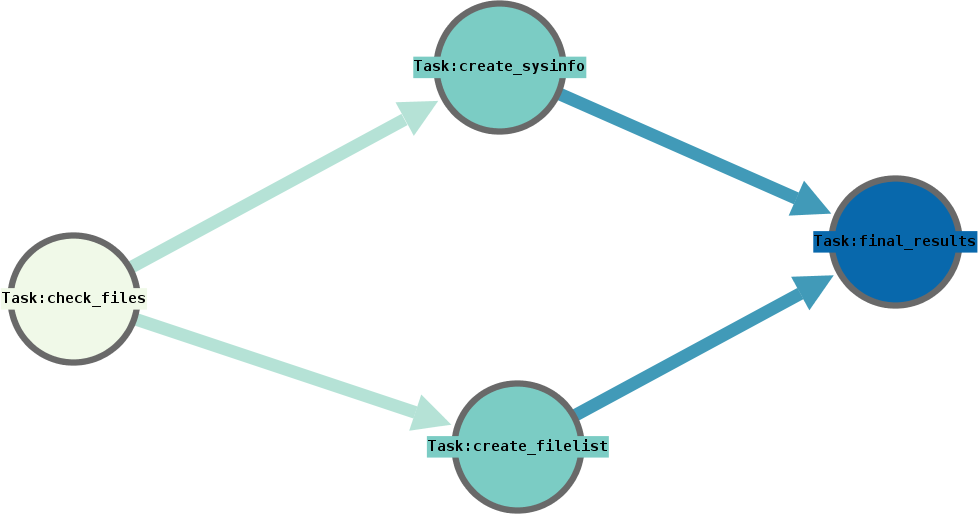
\includegraphics[width=0.8\textwidth]{imagenes/workflow_test.png}
\end{center}
\caption{Visualización del flujo de trabajo \emph{test} }
\label{fig:workflow_test}
\end{figure}


En el ejemplo anterior se pueden apreciar los elementos básicos que componen una tarea del flujo de trabajo, los cuales son explicados a continuación:


\begin{itemize}
\item{\texttt{name}: Nombre de la tarea, que es único entre los nombres de las demás tareas del flujo de trabajo.}
\item{\texttt{command}: Comando en sintaxis de Bash que será ejecutado en esta tarea.}
\item{\texttt{depends}: Lista de los nombres de las tareas que necesitan ser ejecutadas antes de que esta tarea pueda ejecutarse.}
\item{\texttt{download\_files}: Lista de los archivos que deben ser descargados después de terminar la ejecución de la tarea.}
\item{\texttt{include\_files}: Lista de los archivos que deben ser subidos al cluster antes de que la tarea sea ejecutada.}
\end{itemize}

Una característica importante de Sweeper que lo hace único a otros sistemas de administración de flujos de trabajo, es la expansión de parámetros. El usuario puede especificar una tarea que se requiera ejecutar con un conjunto predefinido de argumentos. Sweeper calcula todas las combinaciones posibles de parámetros y automáticamente crea una tarea a ejecutarse por cada posible combinaci\'on de parámetros. Esto es de gran utilidad para la ejecución de experimentos y para la ejecución de aplicaciones de barrido de parámetros. Así, en el listado del código \ref{code:forests_2} se muestra un flujo de trabajo que utliza listas de parámetros de donde se generan las combinaciones de argumentos. En la figura \ref{fig:workflow_forests} se encuentra la representación gr\'afica de este flujo de trabajo.

\begin{figure}
\begin{center}
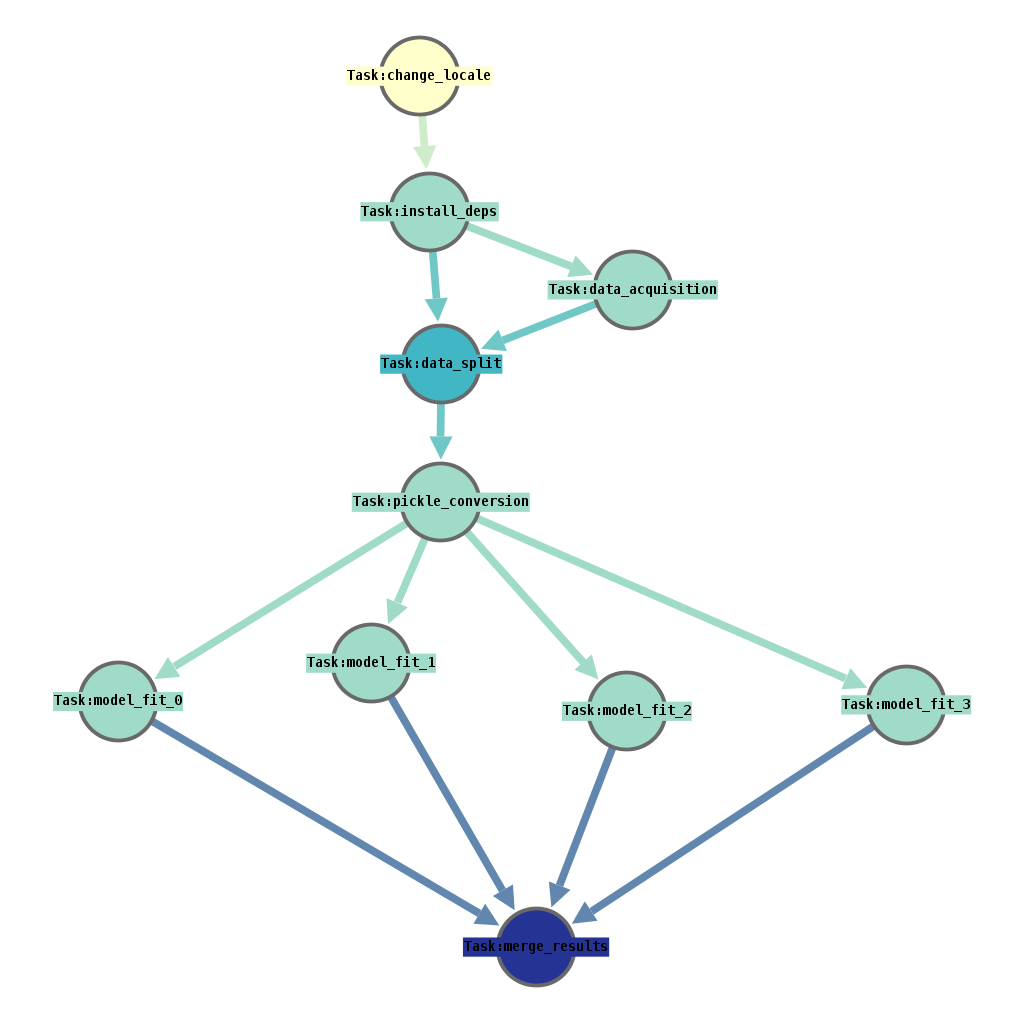
\includegraphics[width=0.8\textwidth]{imagenes/workflow_forests.png}
\end{center}
\caption{Visualización del flujo de trabajo \emph{forests} }
\label{fig:workflow_forests}
\end{figure}

\begin{lstlisting}[label={code:forests_1},caption={Flujo de trabajo para búsqueda de parámetros (parte 1).},float]
workflow:
  - name: change_locale
    command: |
        echo "LC_ALL=en_US.UTF-8" | sudo tee -a /etc/environment;
        echo "LANG=en_US.UTF-8" | sudo tee -a /etc/environment;
        sudo update-locale LANG=en_US.UTF-8 LC_ALL=en_US.UTF-8;

  - name: install_deps
    command: |
        set -o xtrace;
        # scikit-learn
        export DEBIAN_FRONTEND=noninteractive;
        sudo apt-get update;
        sudo apt-get install unzip -y;
        sudo apt-get install build-essential gfortran gcc g++ \
                        python3-dev python3-pip python3-setuptools \
                        python3-numpy python3-scipy python3-matplotlib \
                        libatlas-dev libatlas-base-dev libatlas3gf-base -y;
        sudo update-alternatives --set libblas.so.3 /usr/lib/atlas-base/atlas/libblas.so.3;
        sudo update-alternatives --set liblapack.so.3 /usr/lib/atlas-base/atlas/liblapack.so.3;
        sudo pip3 install -U scikit-learn;
        # doge package
        sudo apt-get install git -y;
        git clone https://github.com/dominoFire/doger.git;
        cd doger;
        sudo pip3 install .;
        cd ..;
    depends: [change_locale]

  - name: data_acquisition
    command: |
        unzip train.csv.zip;
        mv train.csv labeled.csv;
    include_files: [train.csv.zip]
    depends: [install_deps]

  - name: data_split
    command: |
        doger split_traintest labeled.csv 0.70;
        doger split_xy labeled_train.csv Cover_Type;
        doger split_xy labeled_test.csv Cover_Type;
    depends: [data_acquisition, install_deps]

  - name: pickle_conversion
    command: |
        doger csv2pk labeled_train_predictors.csv labeled_train_response.csv;
        doger csv2pk labeled_test_predictors.csv labeled_test_response.csv;
    depends: [data_split]
\end{lstlisting}

\begin{lstlisting}[label={code:forests_2},caption={Flujo de trabajo para búsqueda de parámetros (parte 2).},float]
  - name: model_fit
    command: |
        doger gridsearch \
            labeled_train_predictors.pk labeled_train_response.pk \
            labeled_test_predictors.pk labeled_test_response.pk \
            @config_file \
            obj out;
    depends: [pickle_conversion]
    param_grid:
        config_file: [gridsearch_xt_config.py, gridsearch_rf_config.py, gridsearch_gnb_config.py, gridsearch_bnb_config.py]
    include_files: [gridsearch_xt_config.py, gridsearch_rf_config.py, gridsearch_gnb_config.py, gridsearch_bnb_config.py]

  - name: merge_results
    command: |
        doger merge out;
    depends: [model_fit]
    download_files: [out/AllResults.csv]
\end{lstlisting}


\section{Arquitectura}

En figura \ref{fig:sweeper-arch} se muestra la arquitectura de Sweeper, en donde se pueden los grandes componentes: la ejecución del flujo de trabajo y el planificador. Sweeper utiliza las interfaces de programación de aplicaciones de cada proveedor de servicios de cómputo en la nube para reservar, ejecutar y administrar los recursos utilizados en la nube de cada proveedor. Actualmente, Sweeper puede trabajar con los servicios de cómputo en la nube de Microsoft Azure \cite{microsoft2015azure}. En las siguientes subsecciones, describiremos a detalle cada uno de los componentes de Sweeper.

\begin{figure}
\begin{center}
%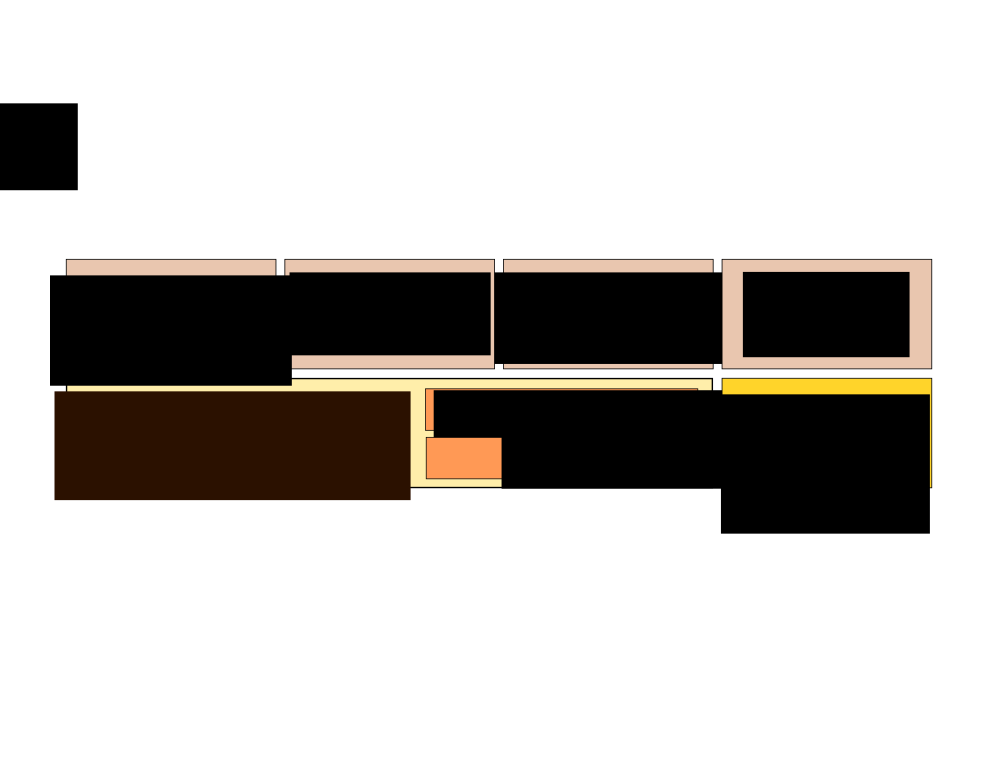
\includegraphics[width=0.8\textwidth]{imagenes/sweeper-architecture.pdf}
\end{center}
\caption{Arquitectura de Sweeper}
\label{fig:sweeper-arch}
\end{figure}


\subsection{Ejecución de flujos de trabajo}

Este componente se encarga de ejecutar el flujo de trabajo en los recursos en la nube de acuerdo a la planificación generada por el componente de planificación. Por el momento, este componente implementa un sistema de colas concurrente en las que las tareas son insertadas y despachadas de acuerdo al tiempo de ejecución estimado.



\subsection{Planifcador}

El planificador busca la asignación de recursos que optimice la calidad en el servicio en la ejecución del flujo de trabajo, interpretado como restricciones de presupuesto o restricciones de fechas límite. 



% \subsection{Perfilador de tareas}

% El perfilador de tareas se utiliza para obtener un modelo de la estimación de tiempos de ejecución independiente de la máquina, el cual es útil para generar planificaciones que optimicen el tiempo total de ejecución o el presupuesto utilizado para la ejecución del flujo de trabajo. A grandes rasgos, el Perfilador de tareas mide el tiempo de ejecución de cada tarea de un flujo de trabajo, guardando un registro de estos tiempos de ejecución junto con los parámetros que se utilizaron para invocar cada tarea.

% Para utilizar el perfilador, hay que invocar Sweeper con la opción \texttt{profile} en la carpeta en donde se encuentre el archivo de flujo de trabajo (\texttt{workflow.yaml}) que se quiera ejecutar, de la siguiente forma:

% \begin{lstlisting}[language=bash]
% $ sweeper profile
% \end{lstlisting}


% \subsection{Perfilador de recursos}

% También, para estimar la velocidad de las máquinas virtuales de un proveedor, sweeper se auxilia del PerfKitBenchmarker, un software diseñado para correr benchmarks, los cuales son pruebas de estrés que ejecutan las máquinas virtuales, cuyos resultados son analizados posteriormente. Para el caso de Sweeper, se utilzan las mediciones de FLOPS que provee el benchmark SPECfp.


\chapter{Resultados}

En este capitulo presentamos algunos resultados del algoritmo ciego y algunas comparaciones con otros algoritmos de planificación. 

Para probar el algoritmo ciego, se generaron aleatoriamente flujos de trabajo utilizando el simulador de flujos de trabajo. El objetivo de estas simulaciones es comparar cuán óptimas son las planificaciones que genera el algoritmo de planificación propuesto en este trabajo respecto a los algoritmos MaxMin, MinMin y Miope. Cabe aclarar que para estas pruebas, el número y el tipo de recursos es determinado por el algoritmo ciego. Luego, utilizando estos recursos sugeridos por el algoritmo ciego, se generan otras planificaciones con los algoritmos MaxMin, MinMin y Miope. También, es importante notar que a todos los algoritmos se les pidió encontrar la planificación con el menor tiempo total de ejecución (makespan). 

Para las pruebas, se generaron 50 flujos de trabajo con 10 tareas cada uno. Los factores de complejidad de las tareas varían entre 50 y 100. Cada flujo de trabajo fue generado con base en un generador de números aleatorios congruencial, utilizando una semilla diferente para cada flujo de trabajo.

Para evaluar el desempeño de los algoritmos de planificación, se tomaron las planificaciones que arrojaba cada algortmo y con ellas, se calculó el makespan y el costo total de ejecución, definido como el producto del costo por hora de mantener una máquina virtual por el periodo de tiempo por el que la máguina se encuentra prendida, es decir, la diferencia entre el tiempo final de la última tarea a ejecutar por la máquina y el tiempo inicial de la primera tarea a ejecutar.





\section{Discusión de resultados}

Esto se debe a que hay algunos detalles con el algoritmo

1) Está pensado para ser más flexible y/o extensible.
2)

\chapter{Conclusiones}
\label{chap:conclusions}

En este trabajo, se propuso un nuevo algoritmo de planificación de flujos de trabajo, tomando en cuenta su ejecución y despliegue en entornos de cómputo en la nube. Este algoritmo, a diferencia de los utilizados para comparar los resultados obtenidos, puede calcular un número mínimo de máquinas o recursos necesarios para correr el flujo de trabajo sin que alguna tarea del flujo de trabajo tenga que esperar por recursos. Otra ventaja de este algoritmo es que se puede utilizar una funci\'on de costo parcial, ya sea para optimizar costo, tiempo de ejecuci\'on u otros requisitos espec\'ificos.

Aunque el algoritmo ciego no genera optimizaciones mucho más eficientes que los algoritmos Miope, MaxMin y MinMin, el algoritmo propuesto en este trabajo da posibilidad a estimar el número de recursos necesarios para ejecutar el flujo de trabajo con máximo paralelismo; los algoritmos utilizados como comparación no realizan la estimación de recursos, solamente minimizan algún costo. Una posible causa de que el algoritmo ciego no tenga mejores resultados que los algoritmos comparados es que no se realiza ninguna optimización a la hora de unir las asignaciones de cada uno de los segmentos. Esto causaría que tareas que son secuenciales puedan ser asignadas a diferentes recursos, incurriendo en un costo adicional por no asignarlos a un solo recurso.

Otra ventaja del algoritmo ciego es su modularidad: es posible cambiar el procedimiento de asignación de tareas a configuraciones de recursos sin afectar la segmentación del flujo de trabajo; también se puede cambiar el procedimiento para unir las asignaciones de todos los segmentos en la planificación final. Finalmente, cabe aclarar que hay algunos flujos de trabajo en donde el algoritmo ciego obtiene mejores resultados de costo de ejecución y tiempo total de ejecución mejores que los resultados obtenidos a través de los algoritmos comparados.

Tambi\'en, en este trabajo se cre\'o un prototipo de un sistema administrador de flujos de trabajo en cómputo en la nube, llamado sweeper, con el objetivo de vislumbrar cu\'ales son las complejidades de construir un sistema de este tipo. Además, sweeper sirvió como una plataforma de prueba a una parte del algoritmo ciego. Sin duda, existen muchos retos t\'ecnicos a solventar, como la administraci\'on de las m\'aquinas virtuales, el almacenamiento y la distribuci\'on de resultados, la configuraci\'on de los programas a ejecutar, entre otros.


\section{Trabajo futuro}

Existen múltiples áreas de oportunidad para mejorar este algoritmo, entre ellas se encuentran:

\begin{enumerate}
\item{Una demostraci\'on formal de que el algoritmo ciego calcula el numero \'optimo de m\'aquinas necesarias para alcanzar el paralelismo no bloqueante.}
\item{Nuevas funciones de costo parcial para evaluar el comportamiento del algoritmo utilizando otras fuentes de optimizaci\'on.}
\end{enumerate}

Por otro lado, el prototipo tiene posibles l\'ineas de trabajo futuro, las cuales se mencionan a continuaci\'on:

\begin{enumerate}
\item{Pooling de m\'aquinas virtuales, debido a que es muy costoso (en t\'erminos de tiempo) prender y apagar m\'aquinas virtuales.}
\item{Entrega progresiva de resultados. El prototipo actual descarga los resultados de la ejecuci\'on una vez que termin\'o el flujo de trabajo; ser\'ia mejor que entregue resultados conforme se vayan obteniendo.}
\item{Perfiladores de recursos y de tareas integrados a sweeper. Los algoritmos de planificación de flujos de trabajo generan mejores asignaciones si conocen con certeza el tiempo de ejecución de las tareas en los recursos disponibles. Si el sistema administrador de flujos de trabajo puede obtener esta información a través del análisis del uso de recursos, entonces podrá hacer mejores asignaciones.}
\item{Utilizar contenedores. Recientemente, la virtualizaci\'on a nivel sistema operativo se ha vuelto popular para desplegar servicios en la nube. Su principal caracter\'istica es que pueden crearse m\'as r\'apido que una m\'aquina virtual y que pueden funcionar con un \emph{kernel} compartido.}
\end{enumerate}


%\appendix
%\chapter{Resultados de ejecución}

\section{Tiempos totales de ejecución}


% latex table generated in R 3.3.1 by xtable 1.8-2 package
% Tue Nov  1 23:39:33 2016
\begin{longtable}{rrrrrrr}
  \hline
N & Nodos & Aristas & Ciego & MaxMin & MinMin & Miope \\ 
  \hline
  0 &  33 &  48 & 13.09 & 3.70 & 3.56 & 5.71 \\ 
    1 &  13 &  22 & 6.06 & 4.15 & 4.41 & 4.70 \\ 
    2 &  44 &  96 & 9.83 & 3.64 & 3.86 & 5.64 \\ 
    3 &  31 &  38 & 6.73 & 2.22 & 2.14 & 2.81 \\ 
    4 &  49 &  95 & 13.83 & 2.05 & 2.11 & 4.48 \\ 
    5 &  33 &  63 & 10.78 & 4.35 & 4.52 & 7.71 \\ 
    6 &  32 &  47 & 8.37 & 2.47 & 2.70 & 3.25 \\ 
    7 &  12 &  18 & 6.78 & 4.43 & 4.22 & 5.12 \\ 
    8 &  31 &  52 & 10.74 & 3.11 & 2.99 & 4.63 \\ 
    9 &  50 &  97 & 19.22 & 5.12 & 5.06 & 8.56 \\ 
   10 &  50 &  72 & 7.87 & 1.32 & 1.33 & 2.43 \\ 
   11 &  36 &  76 & 9.93 & 3.35 & 3.67 & 6.34 \\ 
   12 &  47 & 104 & 16.72 & 2.94 & 3.12 & 6.98 \\ 
   13 &  28 &  30 & 6.92 & 1.15 & 1.19 & 2.76 \\ 
   14 &  39 &  62 & 10.74 & 3.25 & 3.38 & 4.28 \\ 
   15 &  26 &  33 & 5.26 & 1.72 & 1.70 & 2.88 \\ 
   16 &   8 &  11 & 4.27 & 2.58 & 2.88 & 3.84 \\ 
   17 &   4 &   3 & 2.16 & 1.23 & 1.57 & 1.63 \\ 
   18 &   6 &   5 & 2.71 & 2.08 & 1.72 & 1.87 \\ 
   19 &  18 &  19 & 4.61 & 1.59 & 1.66 & 2.32 \\ 
   20 &  24 &  32 & 7.94 & 2.29 & 2.35 & 4.01 \\ 
   21 &  14 &  23 & 5.78 & 3.10 & 3.51 & 3.73 \\ 
   22 &  35 &  96 & 14.96 & 4.93 & 5.35 & 9.08 \\ 
   23 &  15 &  18 & 4.60 & 2.86 & 3.40 & 3.98 \\ 
   24 &   2 &   1 & 1.41 & 1.41 & 1.41 & 1.41 \\ 
   25 &  42 &  78 & 10.50 & 3.90 & 3.75 & 4.36 \\ 
   26 &  24 &  53 & 11.14 & 6.16 & 6.00 & 7.84 \\ 
   27 &  28 &  45 & 9.81 & 2.73 & 2.89 & 4.19 \\ 
   28 &  42 &  94 & 13.19 & 4.21 & 4.74 & 5.85 \\ 
   29 &  42 &  78 & 12.59 & 1.88 & 2.01 & 4.73 \\ 
   30 &   4 &   3 & 2.71 & 2.71 & 2.71 & 2.71 \\ 
   31 &   1 &   0 & 0.76 & 0.76 & 0.76 & 0.76 \\ 
   32 &   3 &   2 & 2.28 & 2.28 & 2.28 & 2.28 \\ 
   33 &  26 &  42 & 7.42 & 1.47 & 1.48 & 2.92 \\ 
   34 &  47 &  61 & 6.24 & 1.17 & 1.12 & 2.44 \\ 
   35 &  30 &  41 & 8.49 & 2.99 & 2.98 & 5.44 \\ 
   36 &  24 &  25 & 5.06 & 2.19 & 2.17 & 2.76 \\ 
   37 &  22 &  52 & 7.38 & 2.66 & 3.01 & 4.54 \\ 
   38 &  28 &  38 & 7.63 & 1.27 & 1.28 & 2.71 \\ 
   39 &  42 &  81 & 11.96 & 3.97 & 4.39 & 6.30 \\ 
   40 &  17 &  23 & 4.26 & 1.52 & 1.52 & 2.66 \\ 
   41 &  48 &  76 & 7.21 & 2.47 & 2.58 & 4.13 \\ 
   42 &  37 &  58 & 11.43 & 4.77 & 5.18 & 6.75 \\ 
   43 &  15 &  16 & 2.66 & 0.94 & 0.93 & 1.39 \\ 
   44 &  27 &  57 & 11.58 & 3.92 & 4.30 & 7.16 \\ 
   45 &  21 &  37 & 7.76 & 4.61 & 4.65 & 5.57 \\ 
   46 &  10 &  13 & 2.95 & 1.38 & 1.30 & 2.30 \\ 
   47 &  20 &  23 & 4.34 & 0.84 & 0.87 & 1.42 \\ 
   48 &  24 &  34 & 7.79 & 3.08 & 3.09 & 3.70 \\ 
   49 &   6 &   6 & 2.65 & 1.95 & 2.12 & 2.72 \\ 
   50 &   5 &   4 & 2.39 & 1.92 & 2.07 & 1.64 \\ 
   51 &  22 &  31 & 4.12 & 1.50 & 1.50 & 2.19 \\ 
   52 &  49 &  85 & 14.19 & 4.13 & 4.17 & 6.12 \\ 
   53 &  32 &  52 & 9.57 & 2.82 & 2.88 & 5.37 \\ 
   54 &  44 &  62 & 8.44 & 1.41 & 1.62 & 2.48 \\ 
   55 &  25 &  45 & 10.72 & 5.86 & 5.90 & 8.10 \\ 
   56 &  23 &  29 & 3.73 & 1.45 & 1.60 & 2.30 \\ 
   57 &   5 &   4 & 1.87 & 1.26 & 1.84 & 1.26 \\ 
   58 &  17 &  22 & 4.80 & 1.69 & 1.83 & 2.31 \\ 
   59 &   6 &   7 & 4.10 & 2.31 & 2.43 & 2.44 \\ 
   60 &  11 &  13 & 4.83 & 3.21 & 3.44 & 3.98 \\ 
   61 &  13 &  17 & 5.68 & 3.35 & 3.95 & 4.68 \\ 
   62 &  46 &  79 & 11.12 & 3.37 & 3.57 & 4.17 \\ 
   63 &  40 &  64 & 15.22 & 4.19 & 4.36 & 6.80 \\ 
   64 &  16 &  20 & 3.99 & 1.60 & 1.49 & 2.44 \\ 
   65 &  20 &  35 & 7.82 & 2.42 & 2.29 & 3.96 \\ 
   66 &   3 &   2 & 1.19 & 0.85 & 1.06 & 1.19 \\ 
   67 &  39 &  63 & 5.73 & 2.06 & 2.21 & 2.84 \\ 
   68 &   7 &   7 & 2.95 & 2.39 & 2.44 & 2.17 \\ 
   69 &   1 &   0 & 0.90 & 0.90 & 0.90 & 0.90 \\ 
   70 &  10 &  11 & 5.70 & 3.32 & 3.82 & 4.52 \\ 
   71 &  44 &  71 & 10.04 & 4.04 & 3.93 & 4.33 \\ 
   72 &  15 &  17 & 5.19 & 2.30 & 2.09 & 2.93 \\ 
   73 &  49 &  92 & 13.32 & 4.61 & 4.56 & 5.75 \\ 
   74 &  36 &  67 & 11.09 & 3.39 & 3.38 & 5.02 \\ 
   75 &  36 &  62 & 11.09 & 1.70 & 1.67 & 4.05 \\ 
   76 &  18 &  29 & 6.53 & 2.28 & 2.52 & 3.75 \\ 
   77 &   9 &  11 & 5.15 & 3.33 & 3.08 & 4.00 \\ 
   78 &  35 &  83 & 11.35 & 4.60 & 4.57 & 7.07 \\ 
   79 &  26 &  52 & 6.03 & 1.94 & 2.03 & 3.61 \\ 
   80 &  26 &  44 & 5.71 & 3.04 & 3.17 & 3.97 \\ 
   81 &  48 &  89 & 11.58 & 3.37 & 3.34 & 6.34 \\ 
   82 &  10 &  10 & 2.24 & 0.98 & 0.93 & 1.48 \\ 
   83 &  25 &  29 & 7.02 & 2.56 & 2.60 & 3.75 \\ 
   84 &  40 &  67 & 14.20 & 2.12 & 2.20 & 5.00 \\ 
   85 &  17 &  25 & 5.81 & 2.14 & 2.47 & 3.56 \\ 
   86 &  17 &  20 & 2.94 & 1.31 & 1.35 & 1.76 \\ 
   87 &   8 &   8 & 2.97 & 1.93 & 1.86 & 2.16 \\ 
   88 &  17 &  23 & 4.15 & 1.60 & 1.66 & 2.84 \\ 
   89 &  40 &  69 & 7.86 & 2.67 & 2.62 & 4.44 \\ 
   90 &  45 &  74 & 9.21 & 2.95 & 3.03 & 4.58 \\ 
   91 &  25 &  28 & 4.29 & 1.40 & 1.40 & 1.65 \\ 
   92 &  48 &  79 & 14.87 & 2.77 & 3.10 & 6.44 \\ 
   93 &   9 &  15 & 3.54 & 3.15 & 3.34 & 2.93 \\ 
   94 &   7 &   7 & 4.99 & 2.78 & 2.84 & 3.30 \\ 
   95 &   6 &   5 & 2.02 & 2.06 & 1.81 & 1.82 \\ 
   96 &  17 &  23 & 4.88 & 2.24 & 2.24 & 3.68 \\ 
   97 &   6 &   7 & 3.61 & 1.93 & 2.29 & 2.33 \\ 
   98 &   4 &   3 & 2.54 & 1.56 & 1.71 & 2.06 \\ 
   99 &  44 &  81 & 14.15 & 4.19 & 4.22 & 7.42 \\ 
   \hline
\caption{Tiempos totales de planificación estimado por cada algoritmo de planificación.}
\label{table:makespans}
\end{longtable}


\section{Costos de ejecución}

% latex table generated in R 3.3.1 by xtable 1.8-2 package
% Tue Nov  1 23:57:33 2016
\begin{longtable}{rrrrrrr}
  \hline
N & Nodos & Aristas & Ciego & MaxMin & MinMin & Miope \\ 
  \hline
  0 &  33 &  48 & 222.08 & 107.73 & 89.30 & 203.54 \\ 
    1 &  13 &  22 & 41.28 & 28.12 & 29.46 & 31.76 \\ 
    2 &  44 &  96 & 182.59 & 92.85 & 100.95 & 156.22 \\ 
    3 &  31 &  38 & 136.01 & 73.86 & 65.94 & 109.03 \\ 
    4 &  49 &  95 & 194.67 & 117.40 & 111.45 & 402.13 \\ 
    5 &  33 &  63 & 199.90 & 77.74 & 79.12 & 143.12 \\ 
    6 &  32 &  47 & 80.86 & 75.29 & 79.08 & 131.33 \\ 
    7 &  12 &  18 & 45.49 & 29.28 & 23.64 & 34.07 \\ 
    8 &  31 &  52 & 94.04 & 75.18 & 76.41 & 162.05 \\ 
    9 &  50 &  97 & 193.71 & 167.18 & 164.07 & 382.43 \\ 
   10 &  50 &  72 & 209.41 & 120.61 & 116.80 & 240.85 \\ 
   11 &  36 &  76 & 195.21 & 89.65 & 86.34 & 173.66 \\ 
   12 &  47 & 104 & 236.99 & 134.56 & 117.31 & 426.98 \\ 
   13 &  28 &  30 & 54.52 & 49.36 & 48.94 & 156.84 \\ 
   14 &  39 &  62 & 155.98 & 88.90 & 80.18 & 154.13 \\ 
   15 &  26 &  33 & 61.58 & 52.19 & 45.98 & 119.76 \\ 
   16 &   8 &  11 & 16.95 & 14.17 & 13.24 & 25.89 \\ 
   17 &   4 &   3 & 10.95 & 8.17 & 7.24 & 10.95 \\ 
   18 &   6 &   5 & 14.58 & 13.74 & 11.49 & 10.76 \\ 
   19 &  18 &  19 & 52.12 & 36.94 & 32.36 & 63.62 \\ 
   20 &  24 &  32 & 71.83 & 57.41 & 57.16 & 125.46 \\ 
   21 &  14 &  23 & 29.94 & 25.98 & 24.96 & 35.74 \\ 
   22 &  35 &  96 & 267.08 & 86.49 & 90.73 & 171.75 \\ 
   23 &  15 &  18 & 34.04 & 26.76 & 26.26 & 40.21 \\ 
   24 &   2 &   1 & 3.24 & 3.24 & 3.24 & 3.24 \\ 
   25 &  42 &  78 & 220.44 & 100.68 & 95.30 & 121.93 \\ 
   26 &  24 &  53 & 96.73 & 61.65 & 51.16 & 82.94 \\ 
   27 &  28 &  45 & 106.60 & 73.76 & 75.76 & 139.12 \\ 
   28 &  42 &  94 & 340.49 & 111.60 & 121.20 & 169.83 \\ 
   29 &  42 &  78 & 136.32 & 91.43 & 83.66 & 377.24 \\ 
   30 &   4 &   3 & 6.22 & 6.22 & 6.22 & 6.22 \\ 
   31 &   1 &   0 & 1.74 & 1.74 & 1.74 & 1.74 \\ 
   32 &   3 &   2 & 5.25 & 5.25 & 5.25 & 5.25 \\ 
   33 &  26 &  42 & 59.87 & 55.47 & 45.57 & 167.58 \\ 
   34 &  47 &  61 & 109.45 & 99.79 & 103.18 & 251.95 \\ 
   35 &  30 &  41 & 78.83 & 62.94 & 62.02 & 146.22 \\ 
   36 &  24 &  25 & 69.23 & 55.95 & 45.24 & 74.97 \\ 
   37 &  22 &  52 & 146.86 & 48.62 & 54.50 & 85.06 \\ 
   38 &  28 &  38 & 73.08 & 64.31 & 58.48 & 135.28 \\ 
   39 &  42 &  81 & 150.40 & 92.39 & 80.91 & 167.20 \\ 
   40 &  17 &  23 & 43.33 & 34.50 & 34.40 & 72.60 \\ 
   41 &  48 &  76 & 156.63 & 103.04 & 92.15 & 163.37 \\ 
   42 &  37 &  58 & 120.32 & 85.36 & 91.56 & 129.81 \\ 
   43 &  15 &  16 & 46.56 & 28.49 & 27.08 & 33.76 \\ 
   44 &  27 &  57 & 133.50 & 70.44 & 69.27 & 133.98 \\ 
   45 &  21 &  37 & 69.15 & 48.77 & 42.58 & 57.57 \\ 
   46 &  10 &  13 & 32.83 & 22.93 & 23.50 & 37.68 \\ 
   47 &  20 &  23 & 56.86 & 42.30 & 38.29 & 92.06 \\ 
   48 &  24 &  34 & 86.35 & 54.53 & 54.37 & 72.70 \\ 
   49 &   6 &   6 & 17.71 & 12.85 & 9.73 & 16.40 \\ 
   50 &   5 &   4 & 14.92 & 11.68 & 9.53 & 9.74 \\ 
   51 &  22 &  31 & 46.18 & 42.67 & 41.44 & 64.84 \\ 
   52 &  49 &  85 & 310.20 & 147.36 & 135.11 & 243.31 \\ 
   53 &  32 &  52 & 175.38 & 101.20 & 80.82 & 189.08 \\ 
   54 &  44 &  62 & 173.04 & 99.98 & 87.06 & 205.23 \\ 
   55 &  25 &  45 & 72.59 & 54.92 & 54.05 & 90.15 \\ 
   56 &  23 &  29 & 74.12 & 49.83 & 54.34 & 84.72 \\ 
   57 &   5 &   4 & 8.44 & 8.44 & 8.44 & 8.44 \\ 
   58 &  17 &  22 & 43.85 & 38.86 & 32.81 & 60.69 \\ 
   59 &   6 &   7 & 11.16 & 11.80 & 11.16 & 15.69 \\ 
   60 &  11 &  13 & 22.10 & 20.40 & 21.05 & 26.62 \\ 
   61 &  13 &  17 & 63.91 & 37.14 & 34.75 & 52.40 \\ 
   62 &  46 &  79 & 201.23 & 107.03 & 98.60 & 153.92 \\ 
   63 &  40 &  64 & 103.32 & 103.52 & 103.98 & 235.02 \\ 
   64 &  16 &  20 & 46.23 & 38.50 & 33.96 & 59.67 \\ 
   65 &  20 &  35 & 48.95 & 43.61 & 39.46 & 106.08 \\ 
   66 &   3 &   2 & 8.03 & 5.66 & 4.87 & 8.03 \\ 
   67 &  39 &  63 & 110.00 & 75.82 & 78.33 & 126.35 \\ 
   68 &   7 &   7 & 16.36 & 15.36 & 15.71 & 12.99 \\ 
   69 &   1 &   0 & 2.06 & 2.06 & 2.06 & 2.06 \\ 
   70 &  10 &  11 & 30.35 & 21.89 & 21.47 & 28.37 \\ 
   71 &  44 &  71 & 202.38 & 100.48 & 84.79 & 112.55 \\ 
   72 &  15 &  17 & 40.25 & 34.03 & 33.49 & 47.78 \\ 
   73 &  49 &  92 & 152.04 & 116.19 & 102.95 & 166.80 \\ 
   74 &  36 &  67 & 177.57 & 94.41 & 86.38 & 166.23 \\ 
   75 &  36 &  62 & 140.73 & 103.89 & 103.84 & 396.70 \\ 
   76 &  18 &  29 & 74.23 & 35.21 & 40.58 & 70.99 \\ 
   77 &   9 &  11 & 17.57 & 18.75 & 16.59 & 26.67 \\ 
   78 &  35 &  83 & 152.49 & 74.75 & 74.74 & 127.35 \\ 
   79 &  26 &  52 & 65.48 & 48.11 & 47.23 & 110.34 \\ 
   80 &  26 &  44 & 85.60 & 52.41 & 52.48 & 80.43 \\ 
   81 &  48 &  89 & 169.24 & 111.34 & 117.67 & 289.44 \\ 
   82 &  10 &  10 & 18.59 & 15.09 & 14.97 & 26.17 \\ 
   83 &  25 &  29 & 80.35 & 58.72 & 56.02 & 103.90 \\ 
   84 &  40 &  67 & 158.30 & 102.74 & 87.93 & 353.54 \\ 
   85 &  17 &  25 & 78.67 & 37.25 & 42.67 & 63.26 \\ 
   86 &  17 &  20 & 32.03 & 32.55 & 29.90 & 44.78 \\ 
   87 &   8 &   8 & 13.41 & 14.57 & 13.41 & 20.46 \\ 
   88 &  17 &  23 & 34.68 & 34.30 & 32.53 & 48.24 \\ 
   89 &  40 &  69 & 244.55 & 115.28 & 96.31 & 196.25 \\ 
   90 &  45 &  74 & 179.87 & 102.89 & 102.97 & 203.96 \\ 
   91 &  25 &  28 & 56.84 & 50.99 & 50.94 & 68.13 \\ 
   92 &  48 &  79 & 436.54 & 149.46 & 145.51 & 376.05 \\ 
   93 &   9 &  15 & 18.08 & 19.00 & 19.33 & 19.32 \\ 
   94 &   7 &   7 & 29.47 & 18.17 & 13.04 & 22.70 \\ 
   95 &   6 &   5 & 10.79 & 12.95 & 11.18 & 11.89 \\ 
   96 &  17 &  23 & 48.04 & 37.53 & 32.95 & 63.81 \\ 
   97 &   6 &   7 & 20.04 & 12.89 & 10.51 & 15.63 \\ 
   98 &   4 &   3 & 7.87 & 8.49 & 7.87 & 9.59 \\ 
   99 &  44 &  81 & 257.64 & 132.04 & 117.59 & 280.95 \\ 
   \hline
\caption{Costos de ejecución estimados por cada algoritmo de planificación.}
\label{table:costs}
\end{longtable}

\cleardoublepage
\phantomsection
\addcontentsline{toc}{chapter}{Bibliography}

\bibliographystyle{plain}
\bibliography{referencias}
\end{document}
